\addchapheadtotoc
\chapter{Solver Performance}\label{chapter:Example}
The complexity of the radiation solver resulting from both its theoretical foundation as well as its computational implementation calls for an extensive series of validation and performance studies.
Four test geometries are presented in this chapter for verification and profiling using the two methods discussed in section \ref{section:ModelForThisStudy}. The new MCRT models using the bounding volume hierarchy approach will be refered to as MCRT-ArborX, and the model without will be referred to as MCRT-Standard. 
A well-established Fortran implementation developed over the course of many years will be used for comparison, and will be referred to as MCRT-Fort.
The configurations include the canonical one-dimensional plane-parallel medium, a three-dimensional backward-facing step in high temperature flow, a time-accurate turbulent pool fire, and a three-dimensional sooting Pratt \& Whitney aeronautical combustor. 



\section{One dimensional plane-parallel medium}
The plane-parallel medium provides a useful, one dimensional case to test the MCRT code. The geometry consists of two parallel plates surrounding a radiatively-participating medium, as shown in fig. \ref{fig:PlaneParallel}. 
\begin{figure}
\centering
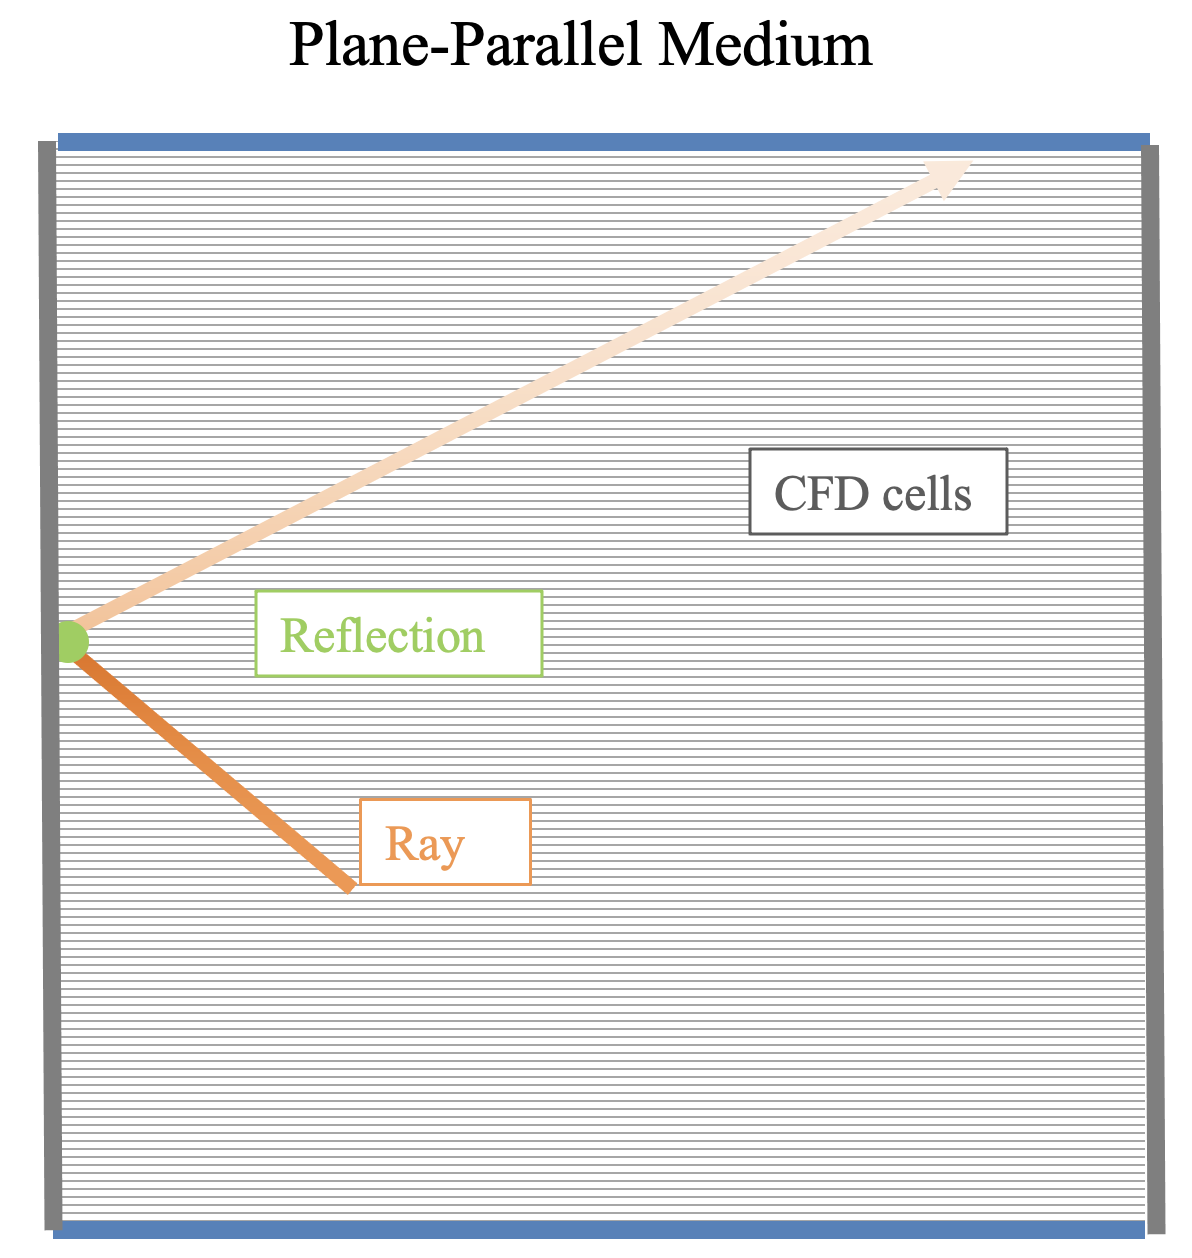
\includegraphics[width=0.5\linewidth]{figures/ch4/PlaneParallel.png}
\caption{Plane parallel medium. Reflective walls are marked in gray, cold-black walls are marked in blue. }
\label{fig:PlaneParallel}
\end{figure}
The system is one-dimensional (implemented into OpenFOAM using ray reflections on the off-axis boundaries). The simulation is steady, and the walls are black-bodies.
Using this configuration, the user can artificially select an absorption coefficient, $\kappa{}$, number of rays emitted per computational cell, N$_r$ medium temperature, $T$, and wall temperatures $T_w$.

Additionally, the relative simplicity of the configuration allows for a reduced-complexity numerical solution which can be used for verification of the solver under variable absorption coefficients and temperatures. Following the derivation from \citet{Modest2013RadiativeTransfer}, eq. \ref{eq:IrrPlaneParallel} defines the irradiance $G$ in $W/m^2$ as a function of optical distance $\tau{}$ between the two plates.
\begin{equation}
    \centering
    G(\tau{})=2\pi{}\left[I_{b1}E_2(\tau{})+I_{b2}E_2(\tau{}_L-\tau{})+\int_0^\tau{}I_b(\tau')E_1(\tau-\tau')d\tau'+\int^{\tau{}_L}_\tau{}I_b(\tau')E_1(\tau'-\tau)d\tau'\right]
    \label{eq:IrrPlaneParallel}
\end{equation}
Where $I_{b1}$ and $I_{b2}$ are the black body intensities from the two plates, and $E_n$ is the exponential integral defined in eq. \ref{eq:ExpInt}.
\begin{equation}
    \centering
    E_n(x)=\int_0^1\mu{}^{n-2}e^{-x/\mu{}}d\mu{}
    \label{eq:ExpInt}
\end{equation}
The absorption in $W/m^3$ at each location can then be evaluated as $\kappa{}G$.

\subsection{Results}
Figures \ref{fig:PPcomp_kappa} to \ref{fig:PPcom_nrays} display comparisons of the MCRT solutions alongside the described analytical implementations for two plates $1$ m apart. The configuration is tested under a variety of absorption coefficients, temperatures, and Monte-Carlo ray counts.
Results show excellent agreement between the MCRT and analytical solutions. The standard deviations of the percent differences between the MCRT and analytical solutions are given in table \ref{table:PPcomp_std}. Little to no variability can be observed throughout the solution across the range of optical thicknesses.
\begin{table}
\centering
\caption{Standard deviations of the percent difference of MCRT and analytical at various absorption coefficients.}
\begin{tabular}{||c c c c c c c c||} 
 \hline
 Absorption Coefficient [m$^{-1}$] & $0.5$ & $1$ & $2$ & $4$ & $6$ & $8$ & $10$\\ [0.5ex] 
 \hline\hline
 $\text{StdDev}\left(\frac{|Q_{rad,MCRT}-Q_{rad,ana}|}{Q_{rad,ana}}\times{100}\right)$ [\%]& $0.27$ & $0.26$ & $0.30$ & $0.37$ & $0.43$ & $0.48$ & $0.52$\\
 \hline
\end{tabular}
\label{table:PPcomp_std}
\end{table}

In fig. \ref{fig:PPcomp_kappa}, it is apparent that higher absorption coefficients result in higher radiative absorption within the medium; however, it should be noted that the increase in absorption coefficient also results in increased emission per eq. \ref{eq:emitting_sphere}. Therefore, there is also a larger degree of available radiation to be absorbed. 
Larger absorption occurs towards the center of the space between the plates due to a greater degree of incident radiation from the emitting medium on both sides.
Towards the edges, radiative absorption decreases due to the absence of radiation from the adjacent cold-black wall.
\begin{figure}[!ht]
\centering
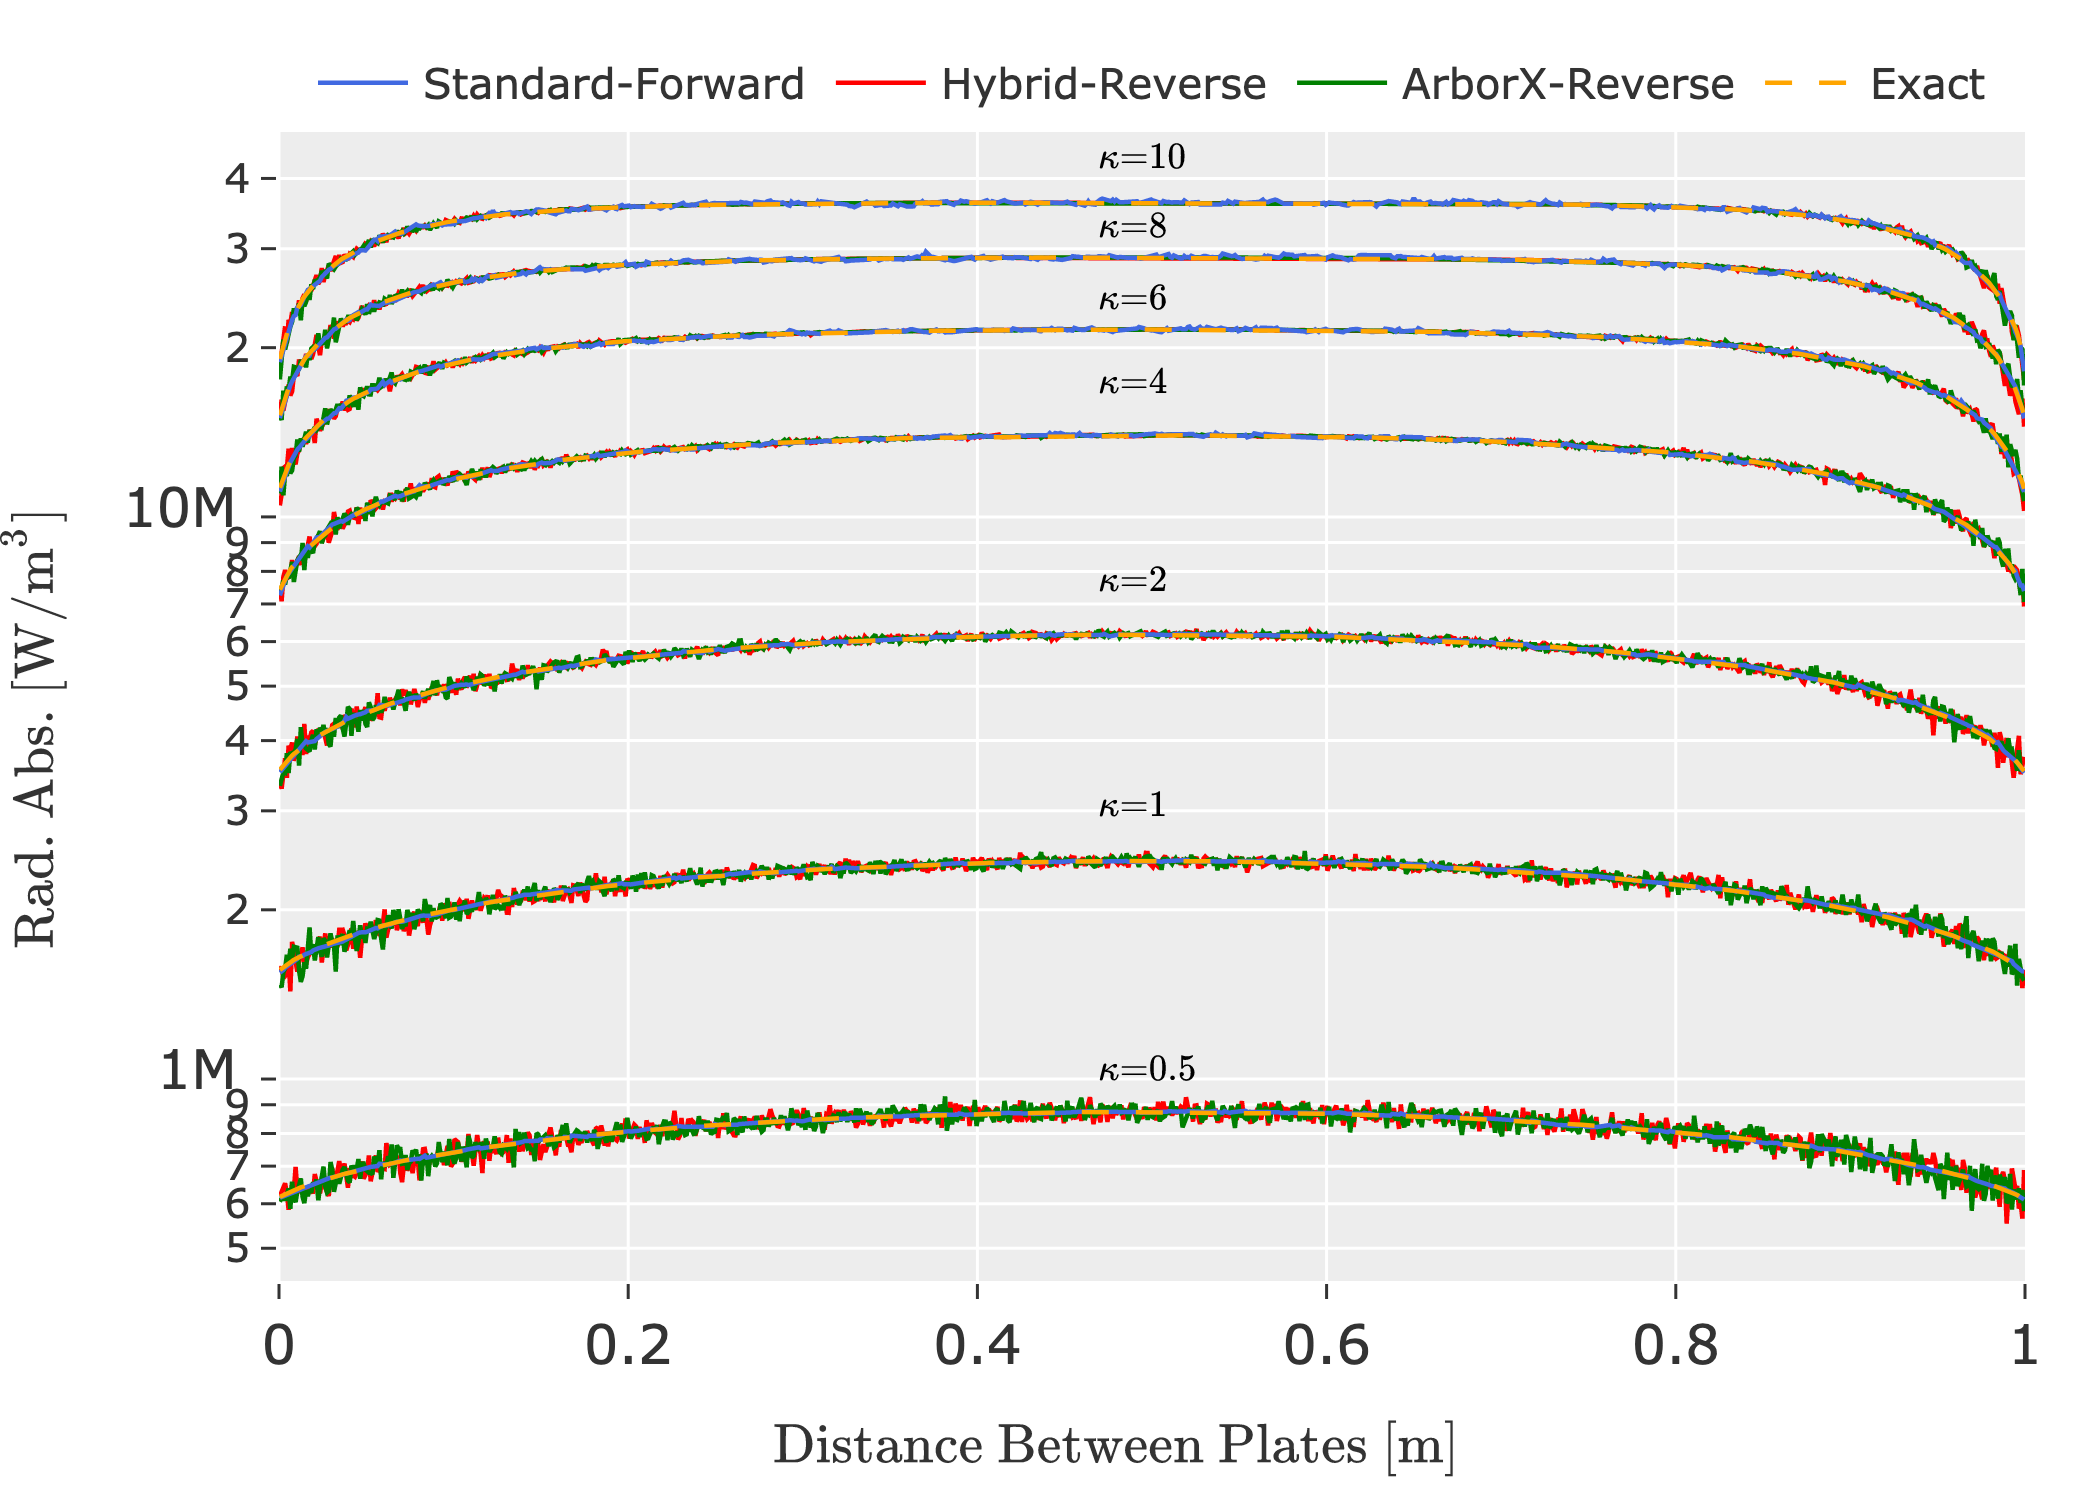
\includegraphics[width=0.95\linewidth]{figures/ch4/PPcomparison1.png}
\caption{Variable absorption coefficient $\kappa{}$ in m$^{-1}$ with T=$2000$K, N$_r$=$1000$, N$_{cells}$=1000.}
\label{fig:PPcomp_kappa}
\end{figure}
\begin{figure}[!ht]
\centering
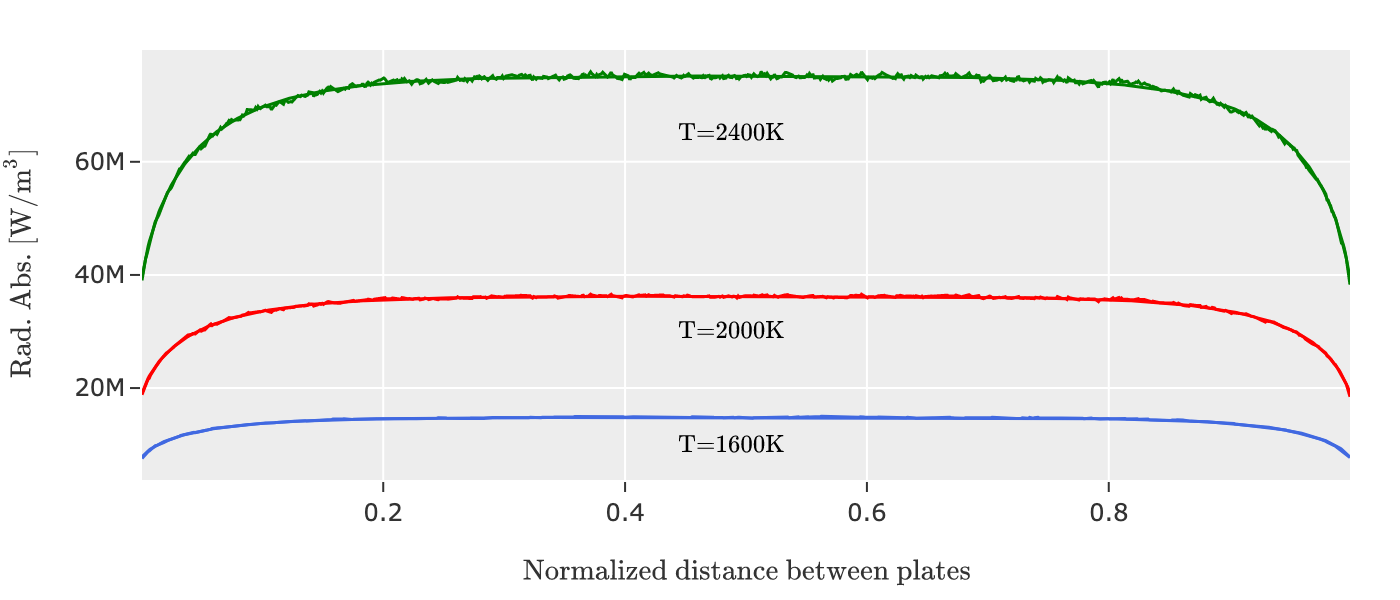
\includegraphics[width=0.95\linewidth]{figures/ch4/PPcomparison2.png}
\caption{Variable temperature with $\kappa{}$=$10$ m$^{-1}$, N$_r$=$1000$, N$_{cells}$=1000.}
\label{fig:PPcomp_temp}
\end{figure}
Temperature also increases radiative absorption, as shown in fig. \ref{fig:PPcomp_temp}. This follows from the fourth order scaling of temperature in the black-body emission function, eq. \ref{eq:PlancksLaw}. An increase in temperature of $400$K approximately doubles the net radiation absorbed.
Finally, as shown in fig. \ref{fig:PPcom_nrays}, lower ray counts show a higher degree of variability, resulting from the stochastic nature of the MCRT method.
The total number of rays traced within the domain scales as $N_r\times{}N_{cells}$. Therefore, an increase in the number of cells can be expected to decrease variability as well.
\begin{figure}
\centering
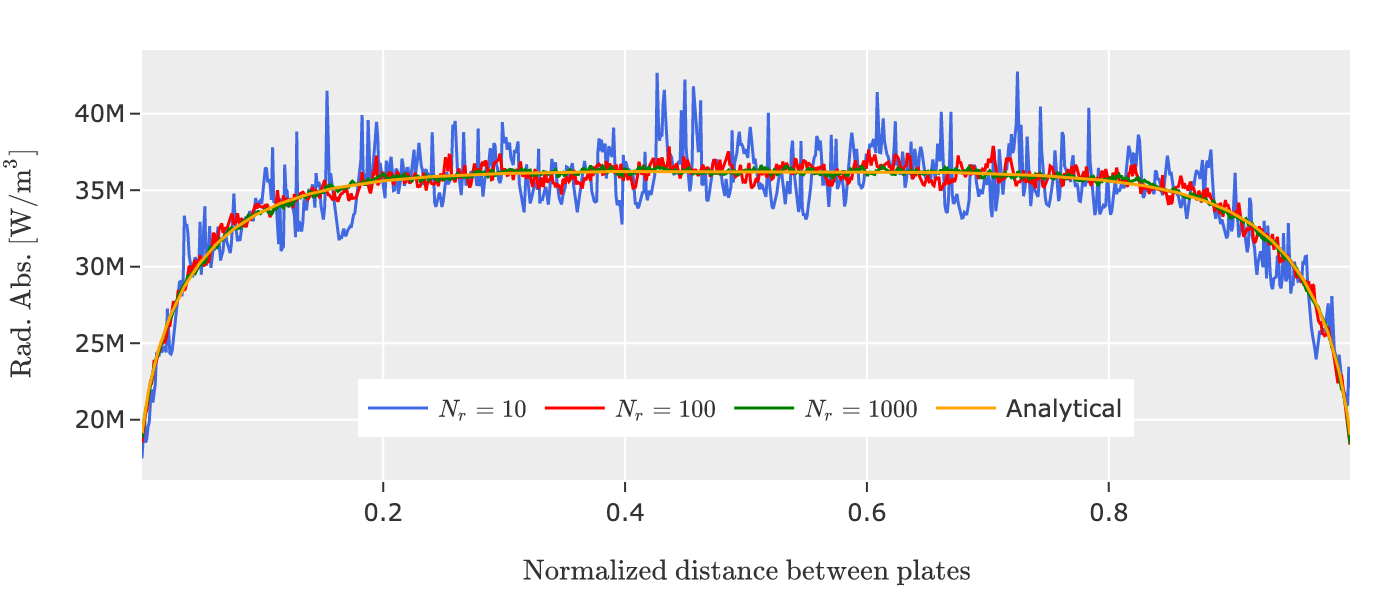
\includegraphics[width=0.95\linewidth]{figures/ch4/PPcomparison3.png}
\caption{Variable number of rays emitted per cell (N$_r$) with $\kappa{}$=$10$ m$^{-1}$, T=$2000$K, N$_{cells}$=1000.}
\label{fig:PPcom_nrays}
\end{figure}

\subsection{Profiling}
Profiling results from the plane-parallel medium were then 

% \begin{figure}



%   \label{fig:PPcomp}
% \end{figure}



\section{Backward-Facing Step Combustor}
The backward-facing step (BFS) combustor is a convenient configuration often used as a simple, repeatable geometry for a variety of studies in fluid dynamics.
Numerous examples exist demonstrating its use for experimental and numerical investigations of turbulent fluid flow~\cite{Armaly1983ExperimentalFlow,Neto1993AStep,Jovic1994Backward-facing5000,Le1997DirectStep}. In contrast, studies of combined turbulent and high temperature flow~\cite{Niemann2016Buoyancy-affectedNumber,Xie2017GeometrySteps}, and reacting flows~\cite{Pouech2021PremixedStep} over backward-facing steps have been modeled significantly less frequently.
In the relatively few studies that exist, the addition of volumetric heating and composition changes resulting from the exothermic chemical reactions have been shown to influence the flow patterns and turbulence intensity of the fluid. 
Recent interest has emerged regarding the relative influence of radiation and convection along the walls many configurations, and the backward-facing step geometry provides a convenient approach for doing so.

\subsection{Case setup}
\begin{figure}
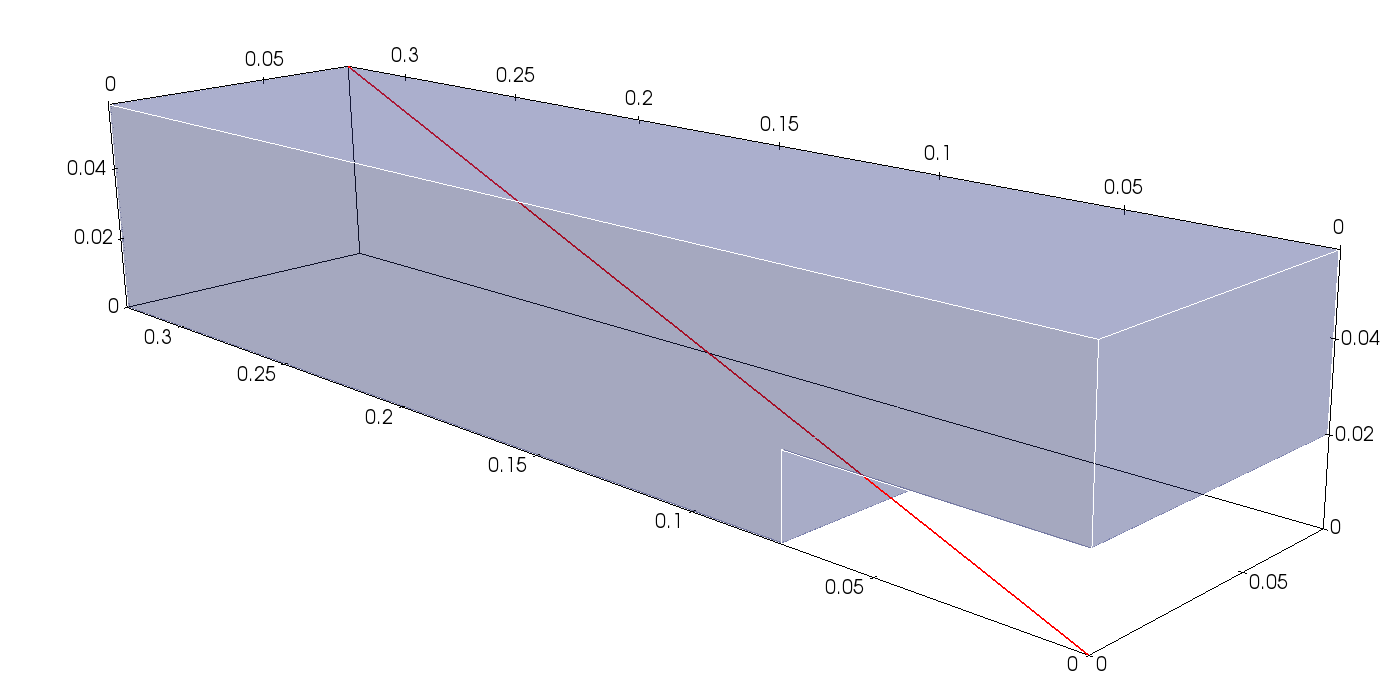
\includegraphics[width=\linewidth]{figures/ch4/BFS_visual.png}
\caption{Dimensions of backward-facing step configuration used in this study in addition to a representative line used to sample radiative properties. All units are in meters. }
\label{fig:BFS_geometry}
\end{figure}

The BFS geometry used in this study is diagrammed in figure \ref{fig:BFS_geometry} based on an experimental configuration at the Pennsylvania State University.
A three-dimensional CFD calculation is intended to be performed for validation with respect to measurements obtained from the experiment. For this case, no chemically reacting flow is included. 
The flow is present in only vitiated form, where a chemical reaction is initiated in a portion of the flow upstream of the step, and the resulting "dirty" air with high CO$_2$ and H$_2$O content is mixed with unreacted air. 
The mixture reaches the main section at an elevated temperature of up to 850K, appreciably lower than expected temperatures of above 2000K when full reactions are present. 
The simulations account for the elevated temperature, but neglect any further chemical reactions beyond the step, resulting in a purely fluid-mechanical and heat-transfer calculation.

Figures \ref{fig:BFS_temperature}, \ref{fig:BFS_streamlines} show temperature and velocity magnitude contours in the BFS. The pressure is atmospheric, and the absorption coefficient is assumed uniform at a value of 0.5 m$^{-1}$ due to the absence of chemical properties in the CFD simulations.

\begin{figure}

\end{figure}
\begin{figure}
  \begin{subfigure}{1\textwidth}
  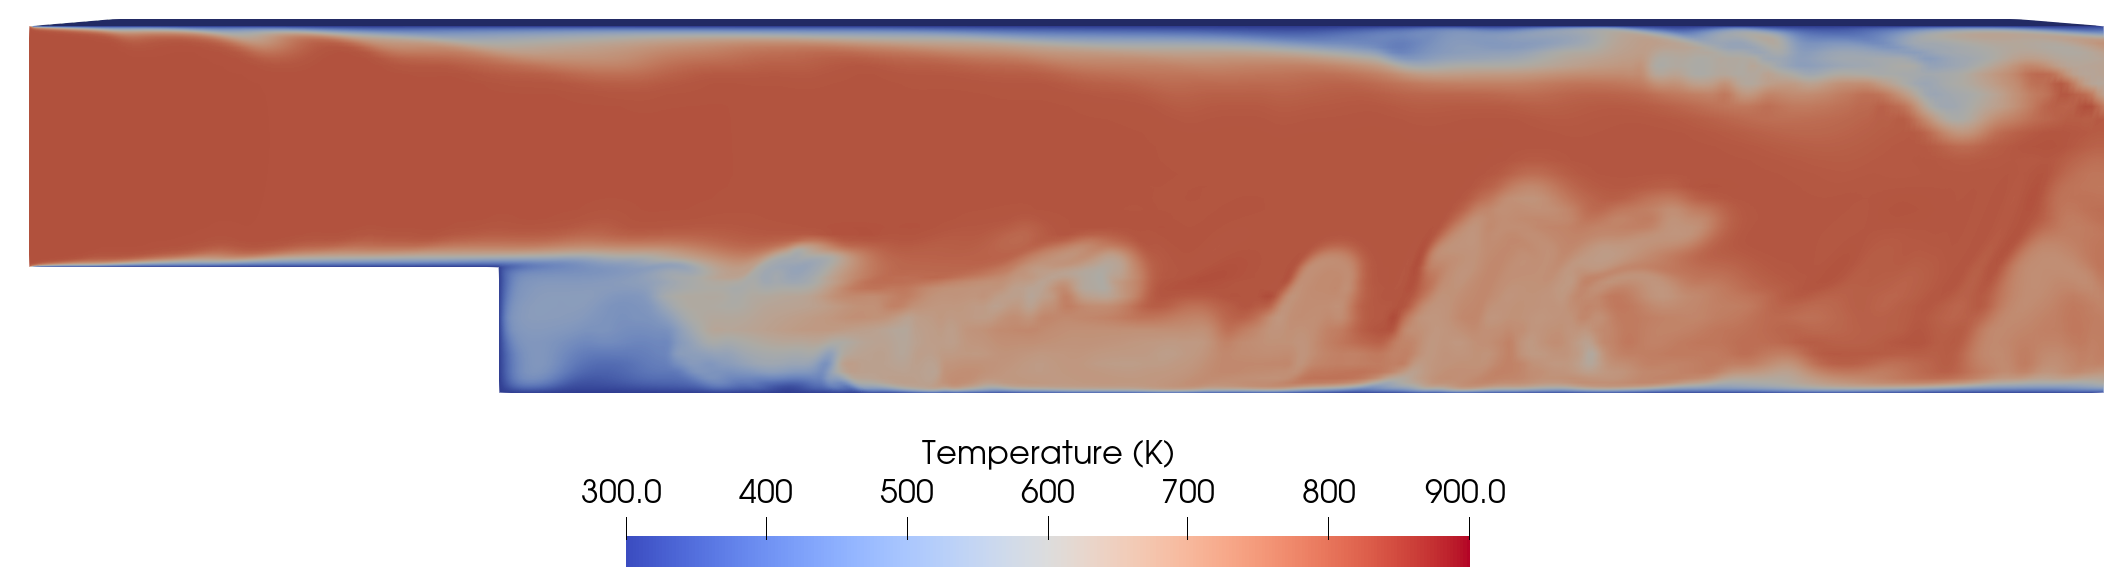
\includegraphics[width=\linewidth]{figures/ch4/BFS_temperature.png}
  \caption{BFS temperature contour along the mid-plane. }
  \label{fig:BFS_temperature}
  \end{subfigure}
  \begin{subfigure}{1\textwidth}
  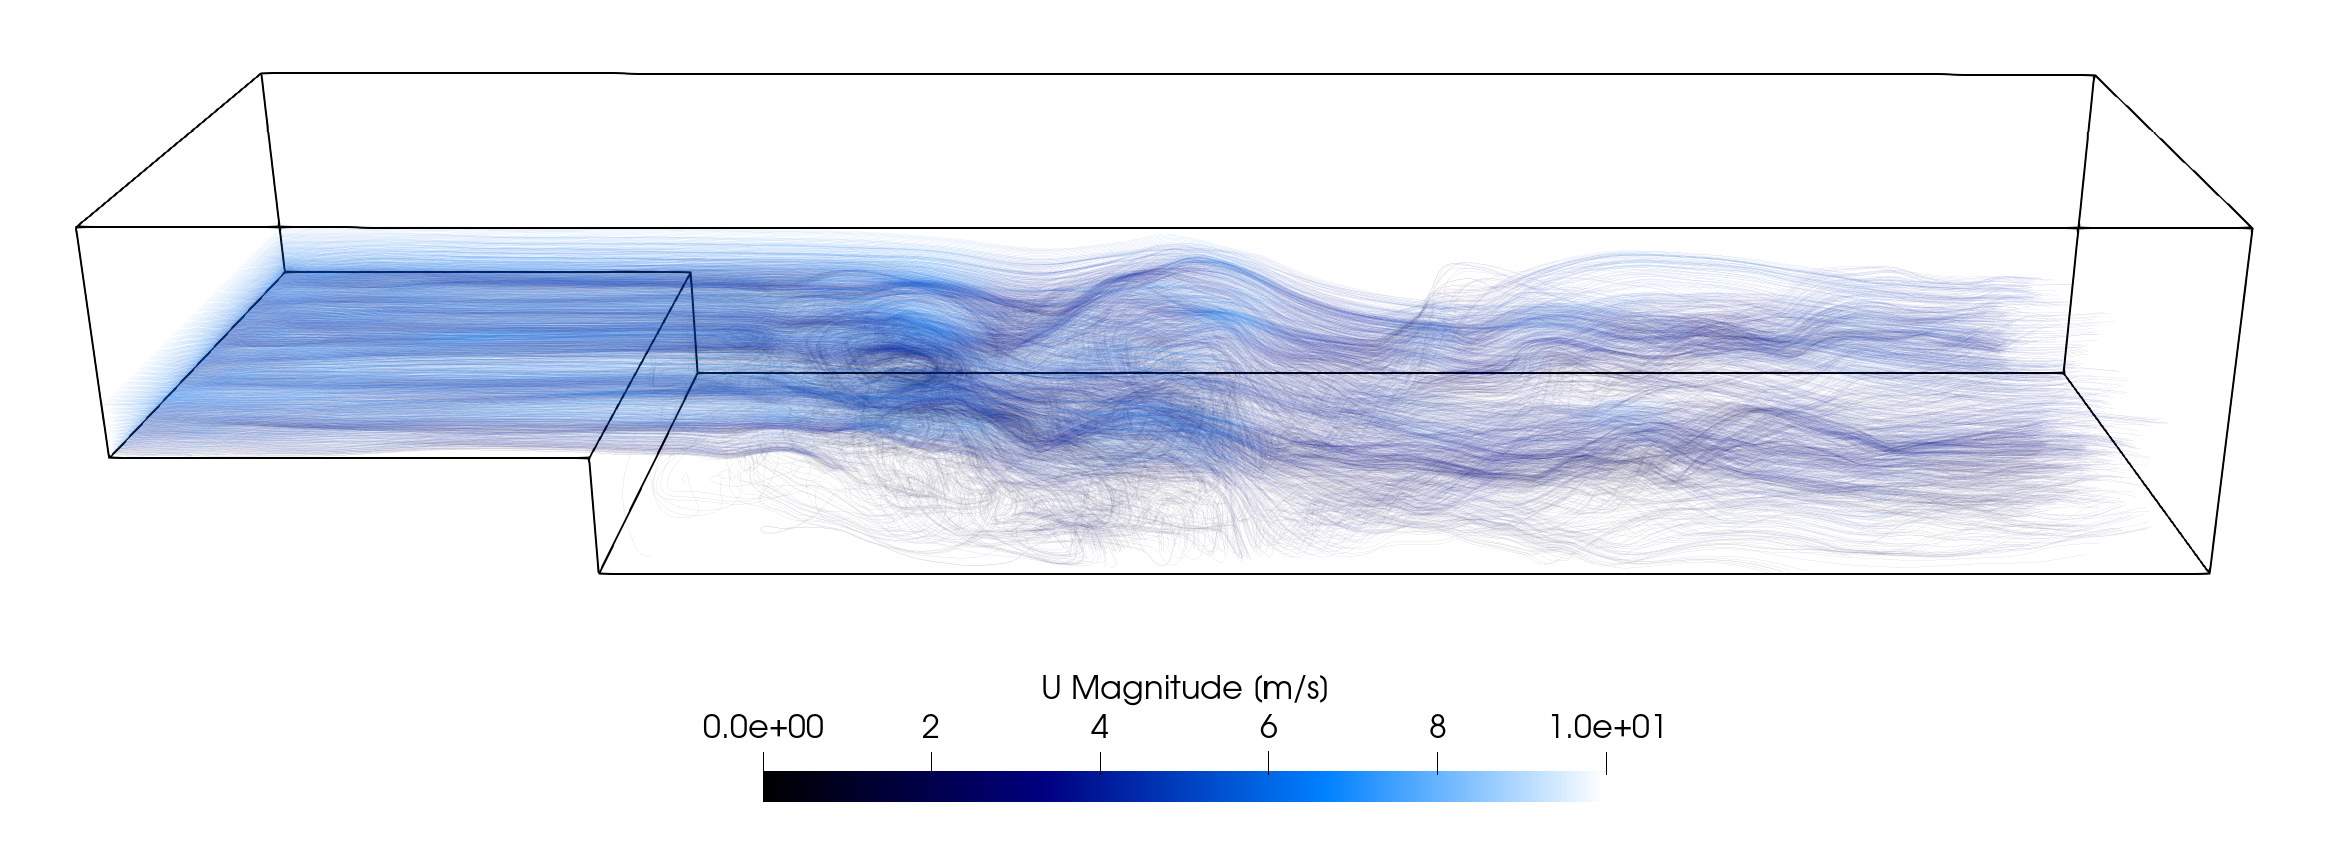
\includegraphics[width=\linewidth]{figures/ch4/BFS_streamlines6.png}
  \caption{Streamlines traced from the entrance of the BFS.}
  \label{fig:BFS_streamlines}
  \end{subfigure}
  \label{fig:BFS_contours}
\end{figure}

\subsection{Results}
A single time-step of the CFD simulation was extracted for a \textit{frozen field analysis} (see chapter \ref{chapter:Introduction}). 
The resulting radiative emission and wall-heat flux iso-contours are shown in figure \ref{fig:BFS_radiationcontours}.
\begin{figure}
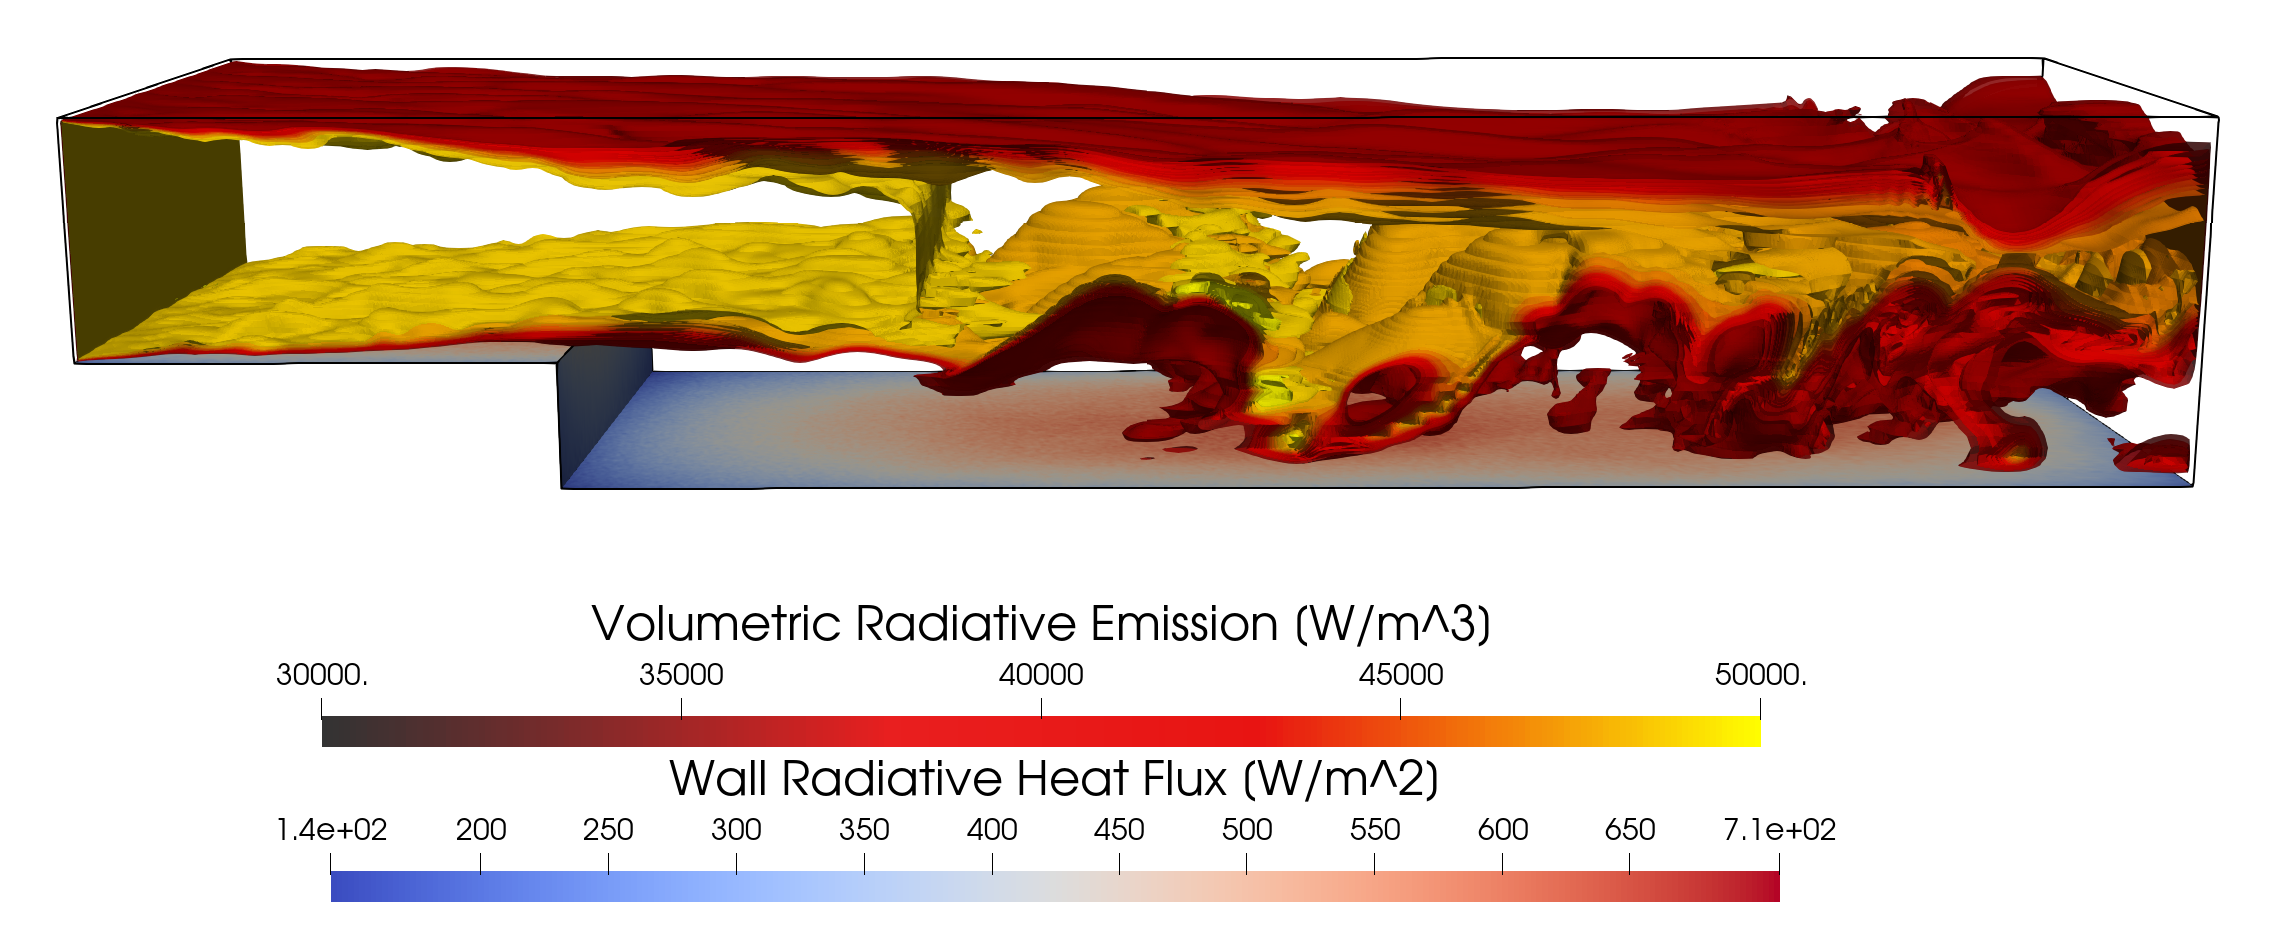
\includegraphics[width=\linewidth]{figures/ch4/BFS_volwallflux3.png}
\caption{Contours of volumetric radiative emission alongside resulting radiative heat flux along the walls.}
\label{fig:BFS_radiationcontours}
\end{figure}
The bulk of radiative emission originates from the re-circulation zone behind the step. Radiation is emitted from the flow and decreases the thermal energy contained in the passing fluid. 
The fluid is then quickly replaced by the new gas at the entrance, which results in a continuous load of radiation incident on the bottom surface of the domain. 

The turbulence present in the recirculation zone is apparent even in the emission contours as a result of the advection of elevated temperatures present. The secondary recirculation zone immediately present adjacent to the step displays lower levels of radiative emission resulting from its slower rate of fresh-gas replenishment.

Figures \ref{fig:BFS_RadAbs}, \ref{fig:BFS_RadEmi}, and \ref{fig:BFS_RadSrc} show the radiative absorption, emission, and net energy source along the line shown in figure \ref{fig:BFS_geometry} using the different solvers for comparison. 
The radiative participation peaks towards the center section of the flame, and results from both the new MCRT implementation closely match results from the established Fortran implementation.

\begin{figure}[!ht]
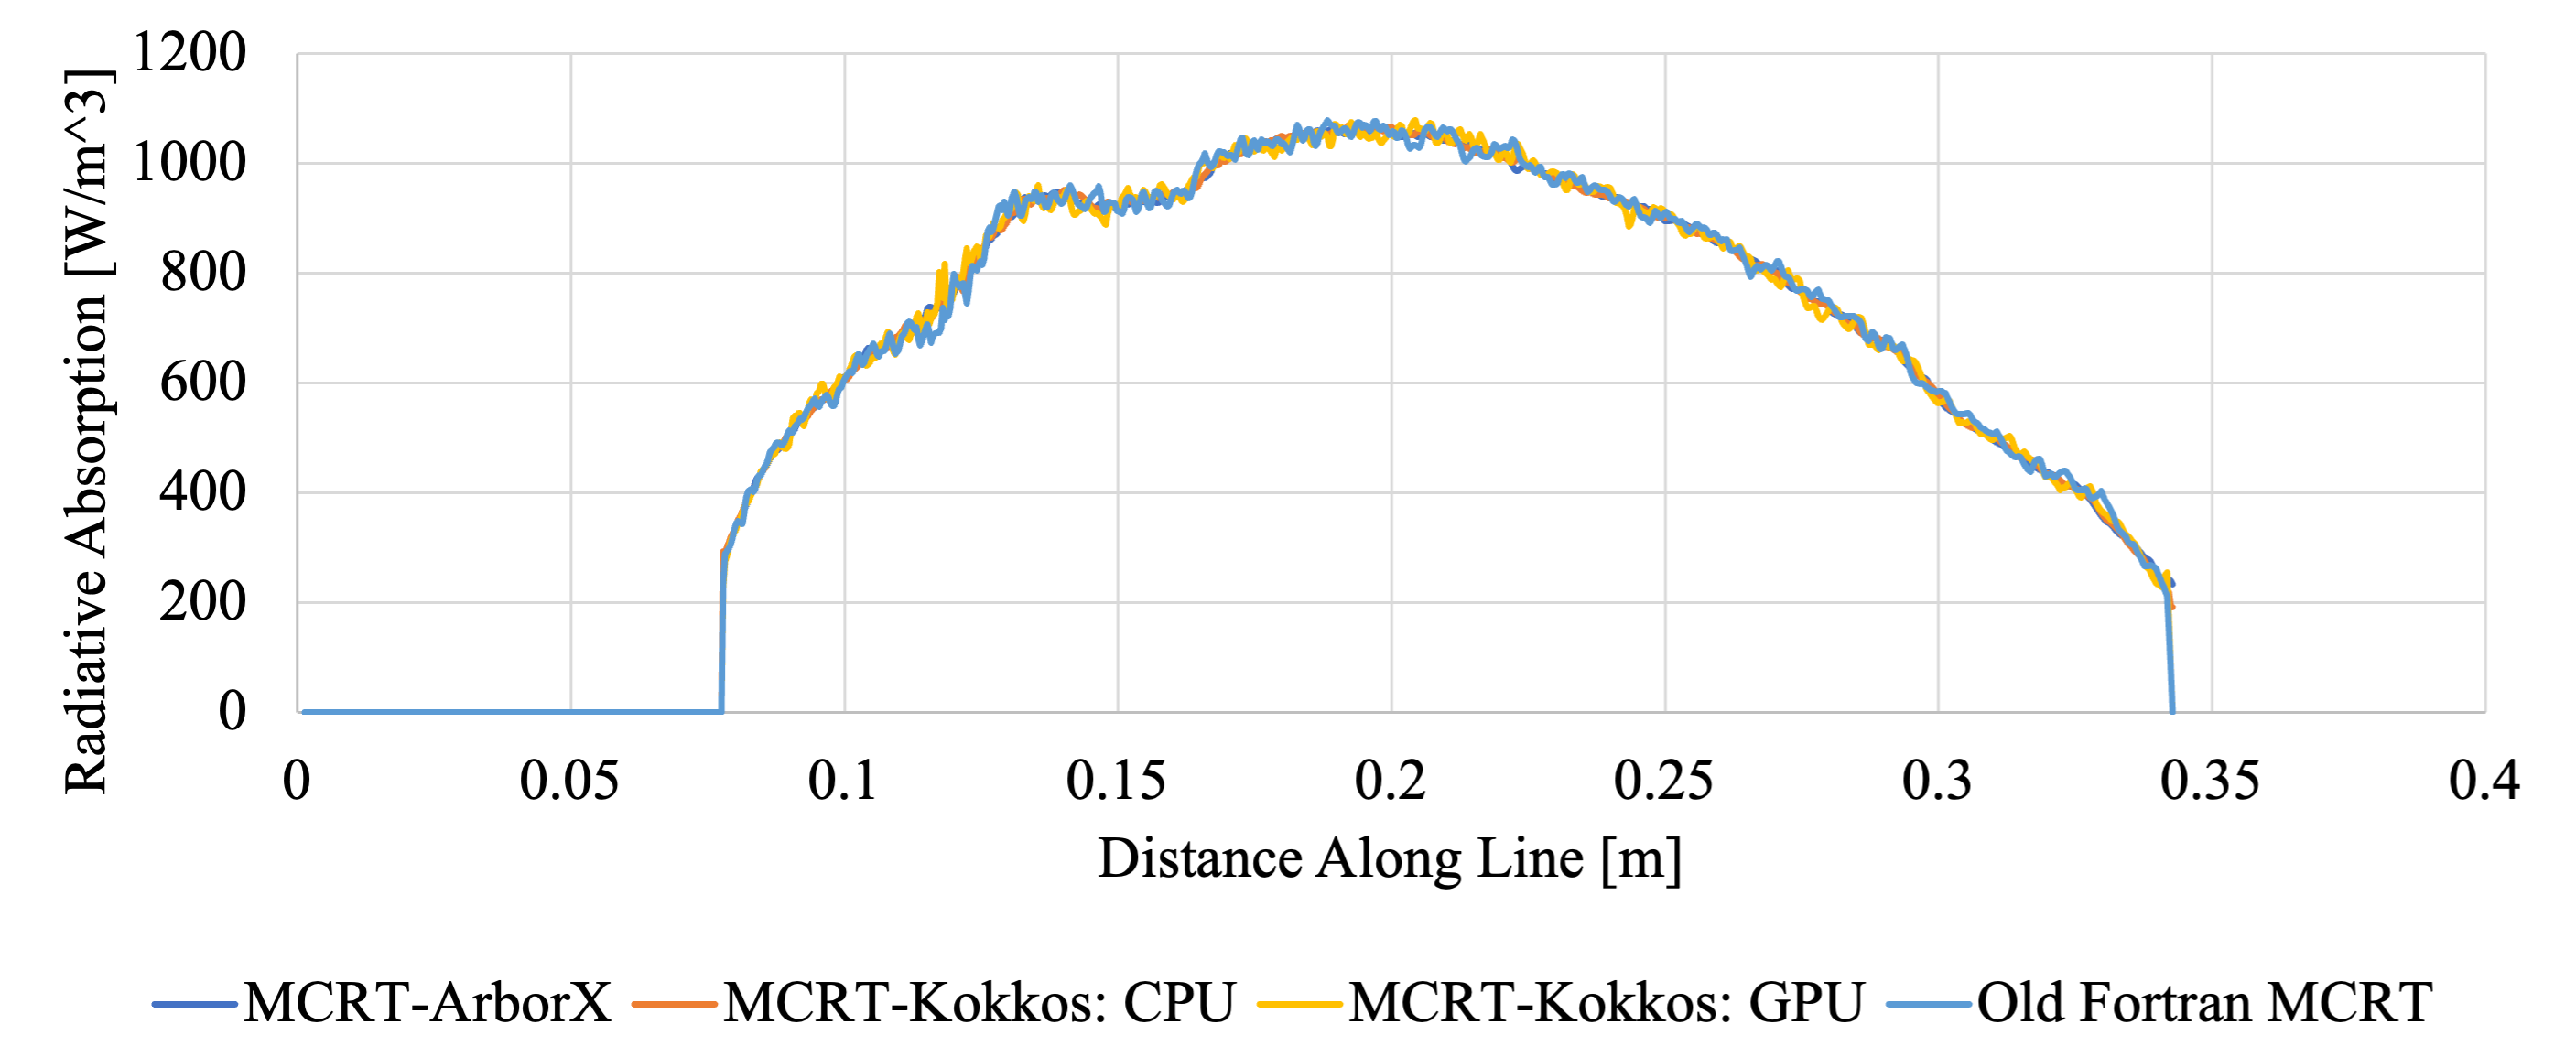
\includegraphics[width=\linewidth]{figures/ch4/LineComparison_RadAbs.png}
\caption{}
\label{fig:BFS_RadAbs}
\end{figure}

\begin{figure}[!ht]
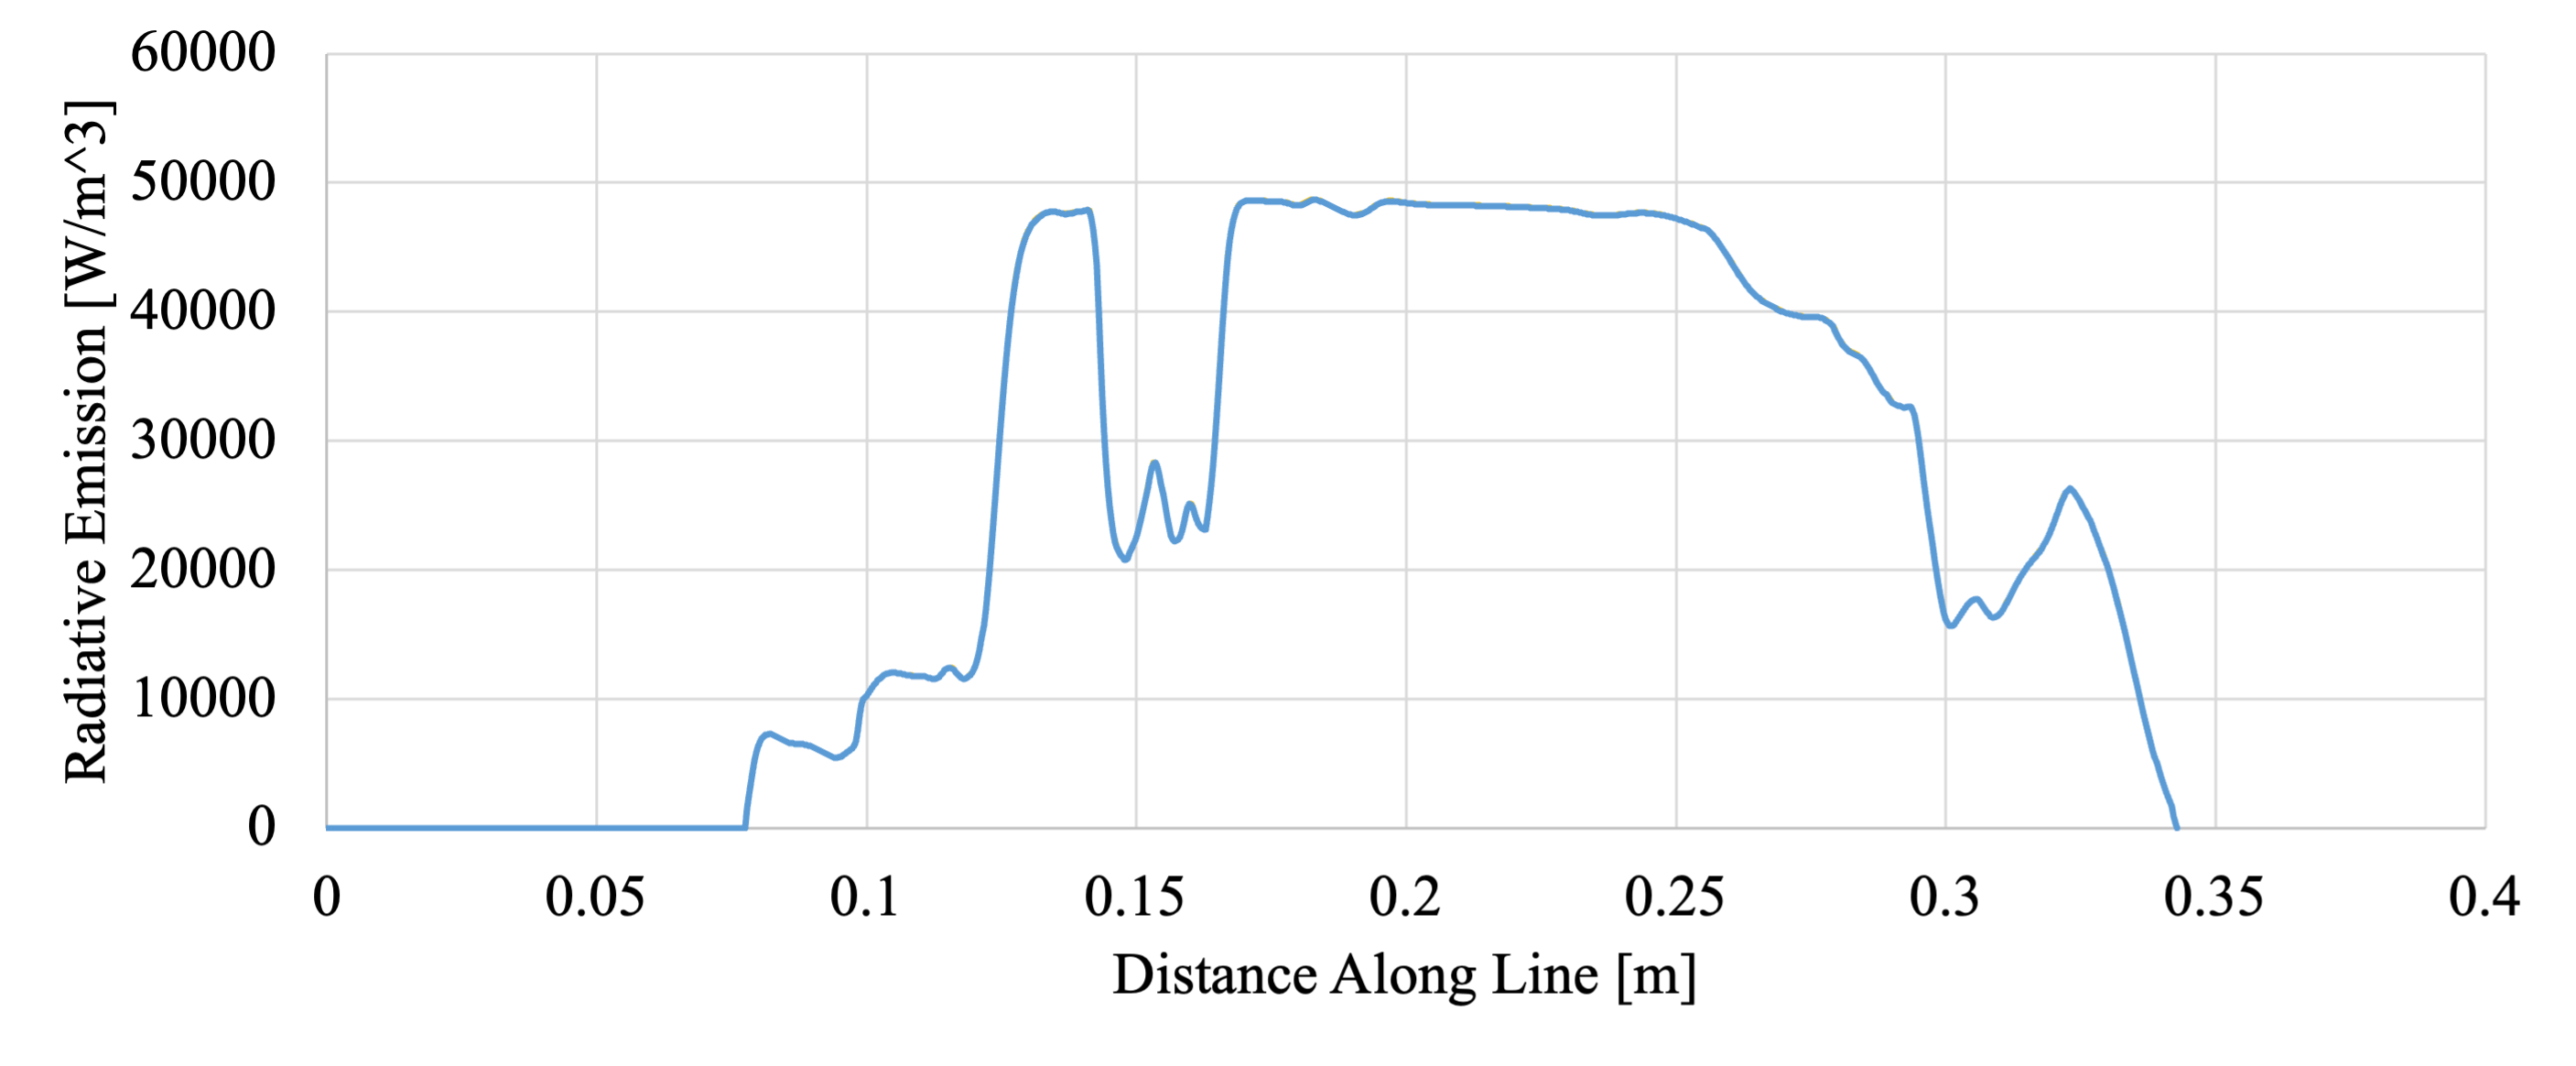
\includegraphics[width=\linewidth]{figures/ch4/LineComparison_RadEmi.png}
\caption{Note: Same legend as in fig. \ref{fig:BFS_RadAbs}. All results overlap exactly.}
\label{fig:BFS_RadEmi}
\end{figure}

\begin{figure}[!ht]
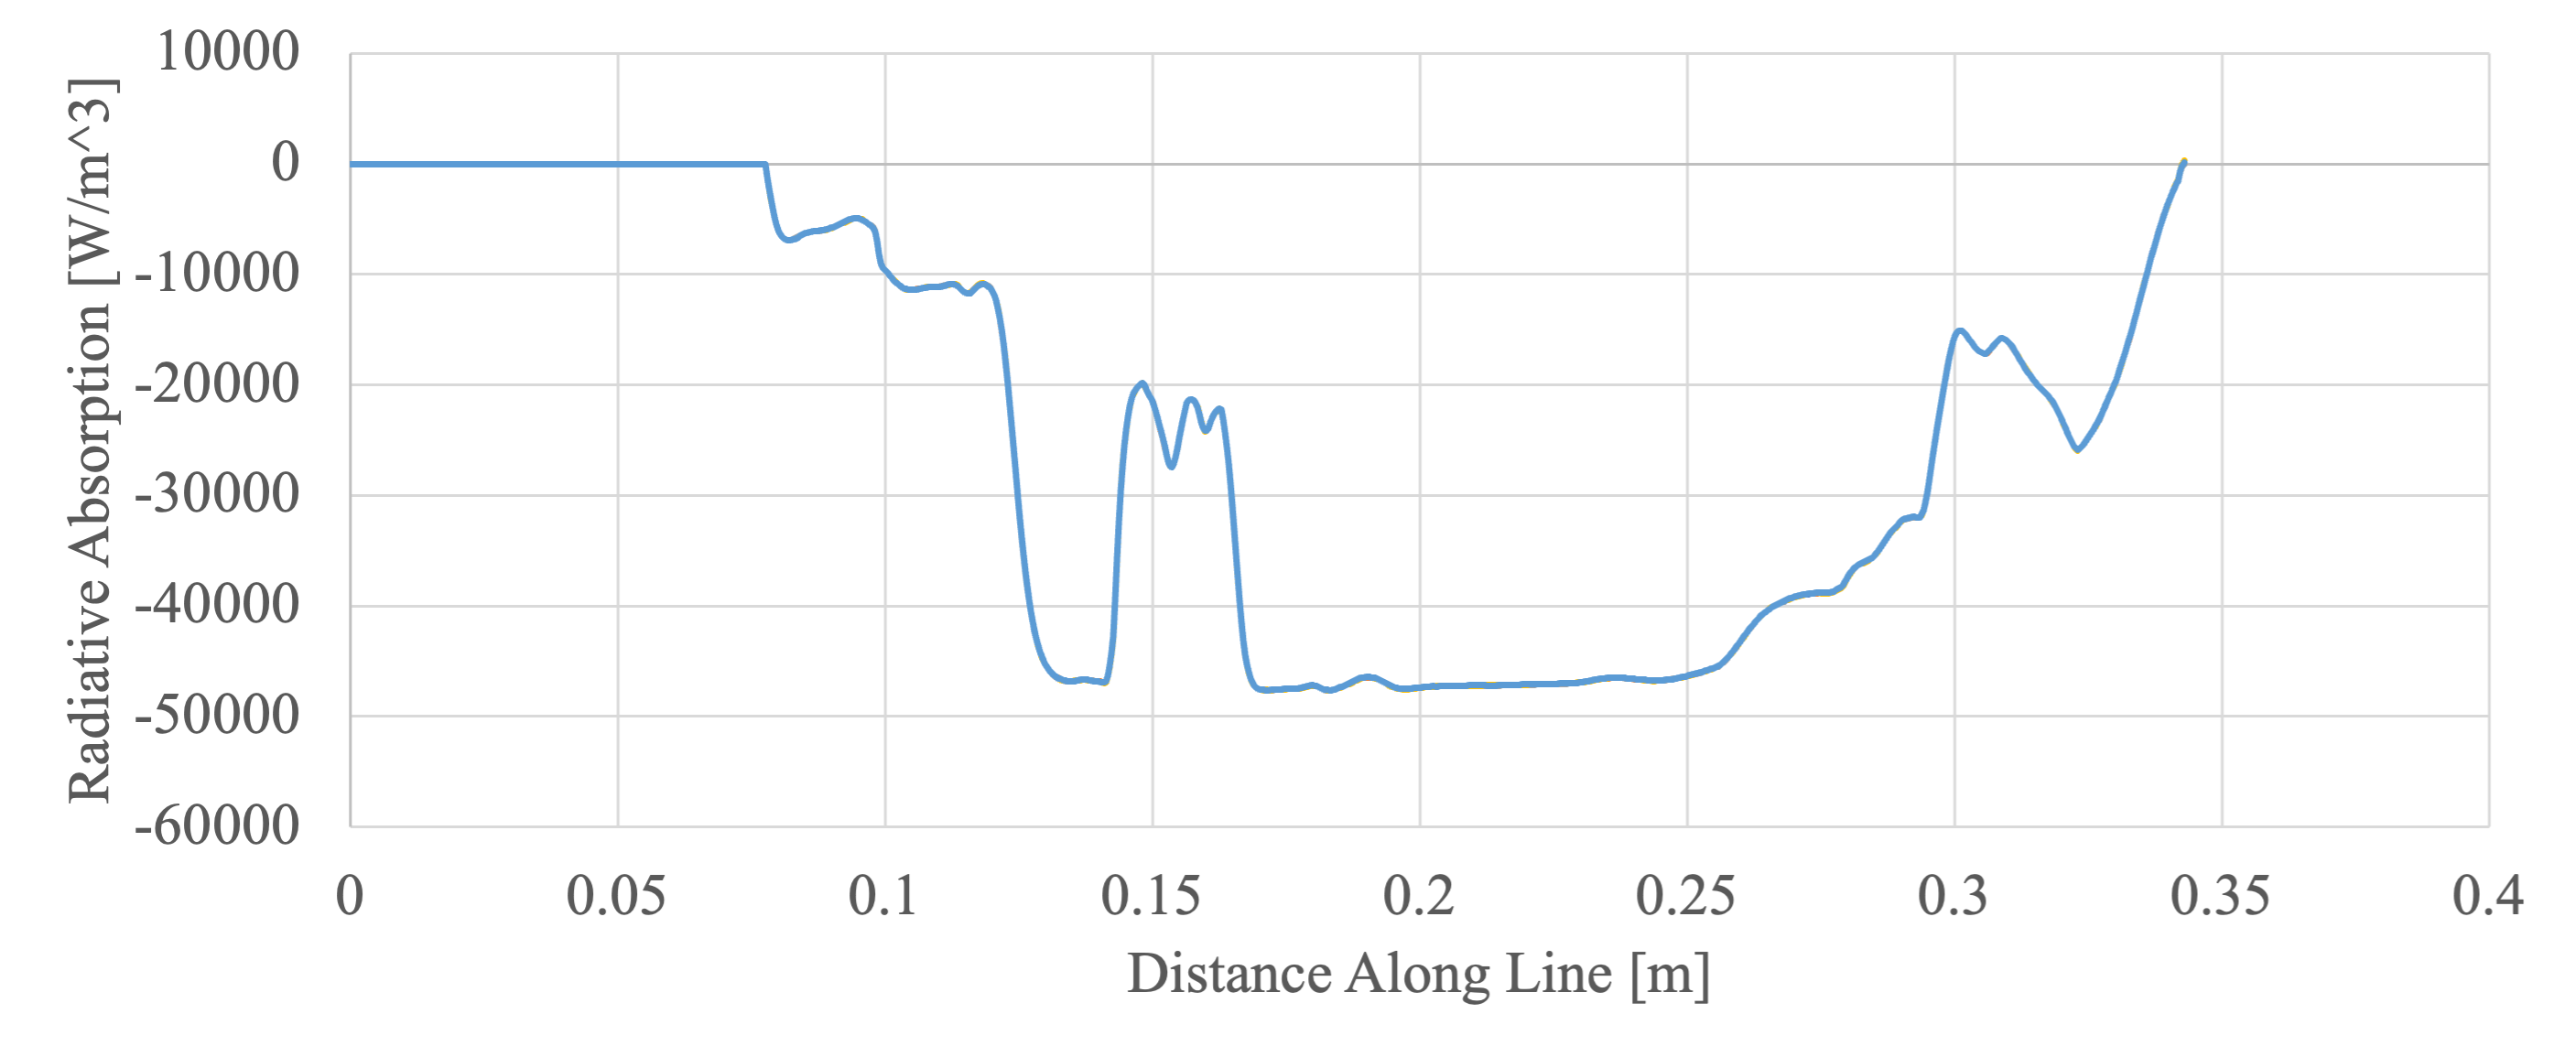
\includegraphics[width=\linewidth]{figures/ch4/LineComparison_RadSrc.png}
\caption{Note: Same legend as in fig. \ref{fig:BFS_RadAbs}. All results overlap exactly.}
\label{fig:BFS_RadSrc}
\end{figure}


\subsection{Model Performance}
The radiation was calculated using both new MCRT models as well as a well-established Fortran-based radiation model for comparison. Simulations were performed at the single time-step using both 1 ray per cell and 10 rays per cell for all solvers, and serial, OpenMP and Cuda were tested as Kokkos backends for the new MCRT. 
Simulations were performed using a 72-core Intel(R) Xeon(R) Gold 5220 CPU shared-memory workstation for OpenMP calculations, and Cuda calculations were performed using NVIDIA V100 GPUs from the high performance computer Narwhal operated by the Naval defense super-computing resource center from the U.S. Department of Defense.

Results are listed in tables \ref{table:BFS_runtime_table_1rpc} and \ref{table:BFS_runtime_table_10rpc} for 1 ray emitted per cell and 10 rays per cell, respectively. The performance of both the MCRT-Kokkos model and the MCRT-ArborX compare extremely well against the MCRT-Fort model for a serial calculation. A runtime improvement of 86\% is already observed before any parallel routines have even been applied.
The dramatic speedup can be attributed to the improved mesh-transfer method implemented in the new MCRT methods. 
Almost no mesh data is duplicated during the mesh transfer process, allowing for minimal delay before the raytracing procedure begins.

\begin{table}[h!]
\centering
\caption{BFS runtime comparisons with 1 ray emitted per CFD cell. The MCRT-Fort parallel procedure is conducted using separate MPI processes within a shared-memory system. The MCRT-Kokkos and MCRT-ArborX run using 30 OpenMP processes.}
\begin{tabular}{||c c c c||} 
 \hline
 Parallel Variation & MCRT-Fort & MCRT-Kokkos & MCRT-ArborX \\ [0.5ex] 
 \hline\hline
 Serial & 2687 s & 376 s & - \\ 
 30 CPU Processors & 52.26 s & 22.5 s & 44.9 \\
 GPU & N/A & 6.91 s & - \\
 \hline
\end{tabular}
\label{table:BFS_runtime_table_1rpc}
\end{table}

\begin{table}[h!]
\centering
\caption{BFS runtime comparisons with 10 rays emitted per CFD cell.}
\begin{tabular}{||c c c c||} 
 \hline
 Parallel Variation & MCRT-Fort & MCRT-Kokkos & MCRT-ArborX \\ [0.5ex] 
 \hline\hline
 30 CPU Processors & 504.37 s & 197.6 s & - \\
 GPU & N/A & 49.1 s & - \\
 \hline
\end{tabular}
\label{table:BFS_runtime_table_10rpc}
\end{table}


The introduction of a parallel CPU implementation also results in dramatic speedups for all three MCRT implementations. MCRT-Fort sees a large speedup not only due to its parallel ray-tracing procedure, but also the long time required to initialize the mesh is reduced resulting from the 30 MPI processes used\footnote{OpenFOAM will load different sections of the mesh on different processors simultaneously when MPI parallelism is used. In this case, the MCRT-Fort code has only been enabled to use MPI parallelism.}.
Within MCRT-Kokkos and MCRT-ArborX, runtimes are decreased as well, but to a lower extent. This can be attributed to the longer mesh initialization time resulting from the usage of a single MPI process.

The usage of a GPU enabled a significant reduction in runtime as well. Speedups of 3.2x and 4x are observed for the 1 ray per cell case and 10 rays per cell case, respectively.
Much of this runtime can be attributed to the transfer of the mesh from the CPU to the GPU.


\section{Small Pool Flame}\label{section:SmallPoolFlame}
The emission of radiation from a buoyant pool flame is of considerable interest to those in the field of fire research. 
The relatively slow fluid motion alongside buoyancy-driven turbulent fluctuations provides a realistic surrogate for many hazardous combustion scenarios such as forest fires and house fires.
The high temperatures from the chemical reaction alongside the larger length scales also provide high radiative emissions alongside high optical thicknesses. 
This results in a system with a high degree of radiation, and is therefore a convenient sample case to demonstrate the use of the present radiation model.

\subsection{Case Setup}
The simulation is based on the \verb|OpenFOAM| tutorial case, smallPoolFlame3D, where mesh refinement has been doubled and the default discrete-ordinates radiation model has been deactivated. 
In the tutorial case, a mass-source is provided through the inlet at the bottom of the domain, where a reaction is also initiated. A turbulent \textbf{premixed?} flame is then simulated with infinitely-fast chemistry for four seconds of physical time.
The simulation is run with radiation enabled, where the net radiation source terms are added to the CFD energy equation solution every timestep.
Both a frozen-field analysis on a single-timestep, and a full transient simulation are conducted and analysed. The single-timestep analysis is conducted using the original smallPoolFlame3D OpenFOAM tutorial case with radiation turned off after 0.8s of physical time; the timestep is shown in fig. \ref{fig:PoolFire_diagram}.

Rays are emitted according to the \textit{adaptive emission} model. In this approach, the number of rays emitted from each computational cell is decided by the emissive power of that cell. Equations \ref{eq:TargetRayEnergy} to \ref{eq:RayEnergies} describe this process, where $E_i$ is the emissive power from cell $i$. 
$N_{rays,tot,target}$ is a user-defined parameter describing the total targeted number of rays to emit throughout the domain.
\begin{equation}
    E_{ray,target}=\frac{\sum^{N_{cells}}_{i}E_{i}}{N_{rays,tot,target}}
    \label{eq:TargetRayEnergy}
\end{equation}
\begin{equation}
    N_{rays,cell,actual}=\frac{E_{i}}{E_{ray,target}}
    \label{eq:NumberOfRays}
\end{equation}
\begin{equation}
    E_{ray,actual}=\frac{E_{i}}{N_{rays,cell,actual}}
    \label{eq:RayEnergies}
\end{equation}


The geometry is a cubic 1$\times$1$\times$1m domain with a grid consisting of 1,728,000 hexahedral cells with 120 divisions per side.
This configuration is studied for both planck-mean gray and line-by-line spectral models, and no Turbulence-Radiation Interaction (TRI) is accounted for in this study.

\begin{figure}
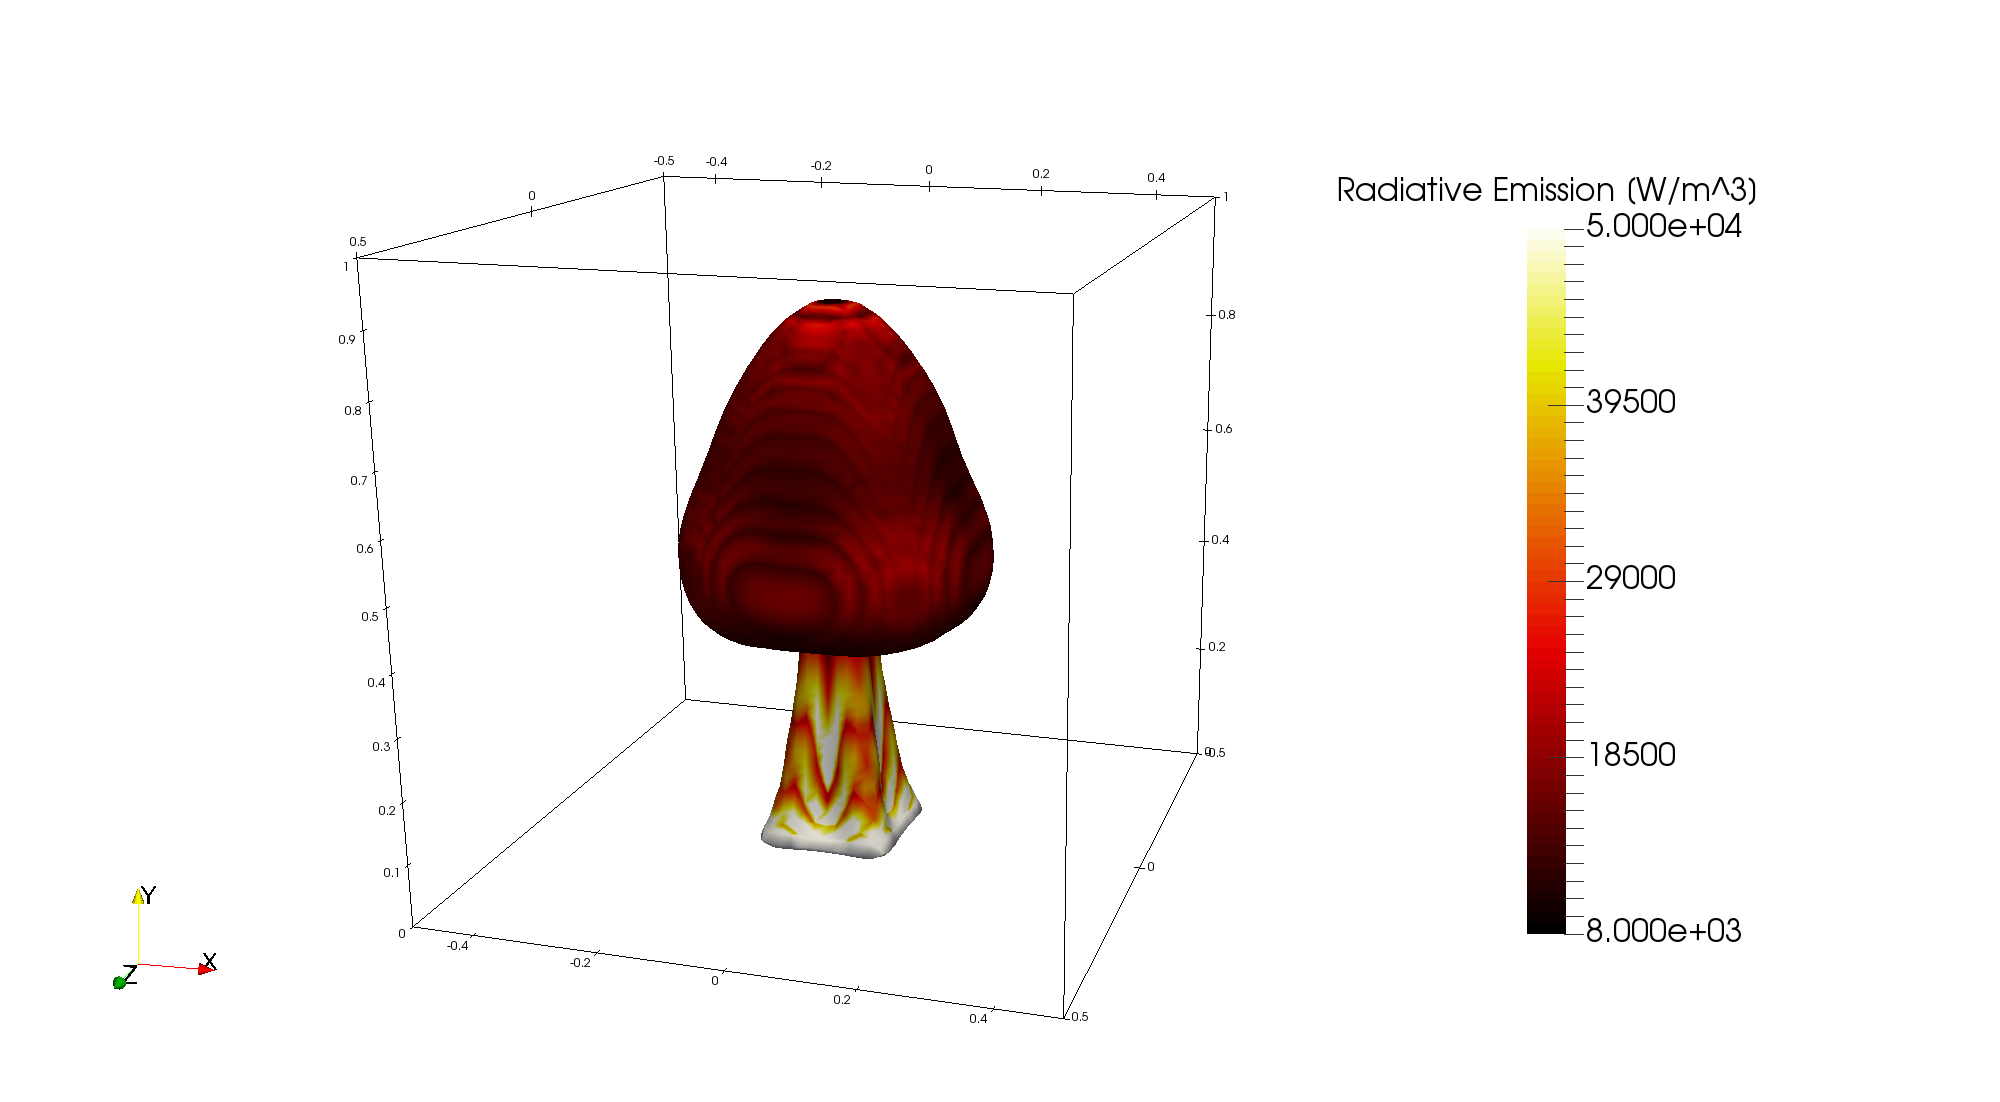
\includegraphics[width=\linewidth]{figures/ch4/contour_early.png}
\caption{An early timestep of the pool fire flame simulation. Isosurface is 0.03 CO$_2$ mass fraction colored by velocity magnitude in meters per second. Axes dimensions are in meters.}
\label{fig:PoolFire_diagram}
\end{figure}

\subsection{Results}
Figure \ref{fig:PoolFire_radiationcontours} displays the radiative emission and wall absorption patterns for the flame. Wall heat flux is maximized near the inlet section, directly adjacent to the location of ignition. 
The radiative emission contours drop towards the outer edges and top section of the mushroom-like shape. The turbulent mixing of the reacting flow with surrounding quiescent fluid results in a reduction in temperature, and lower volumetric emission.  

\begin{figure}
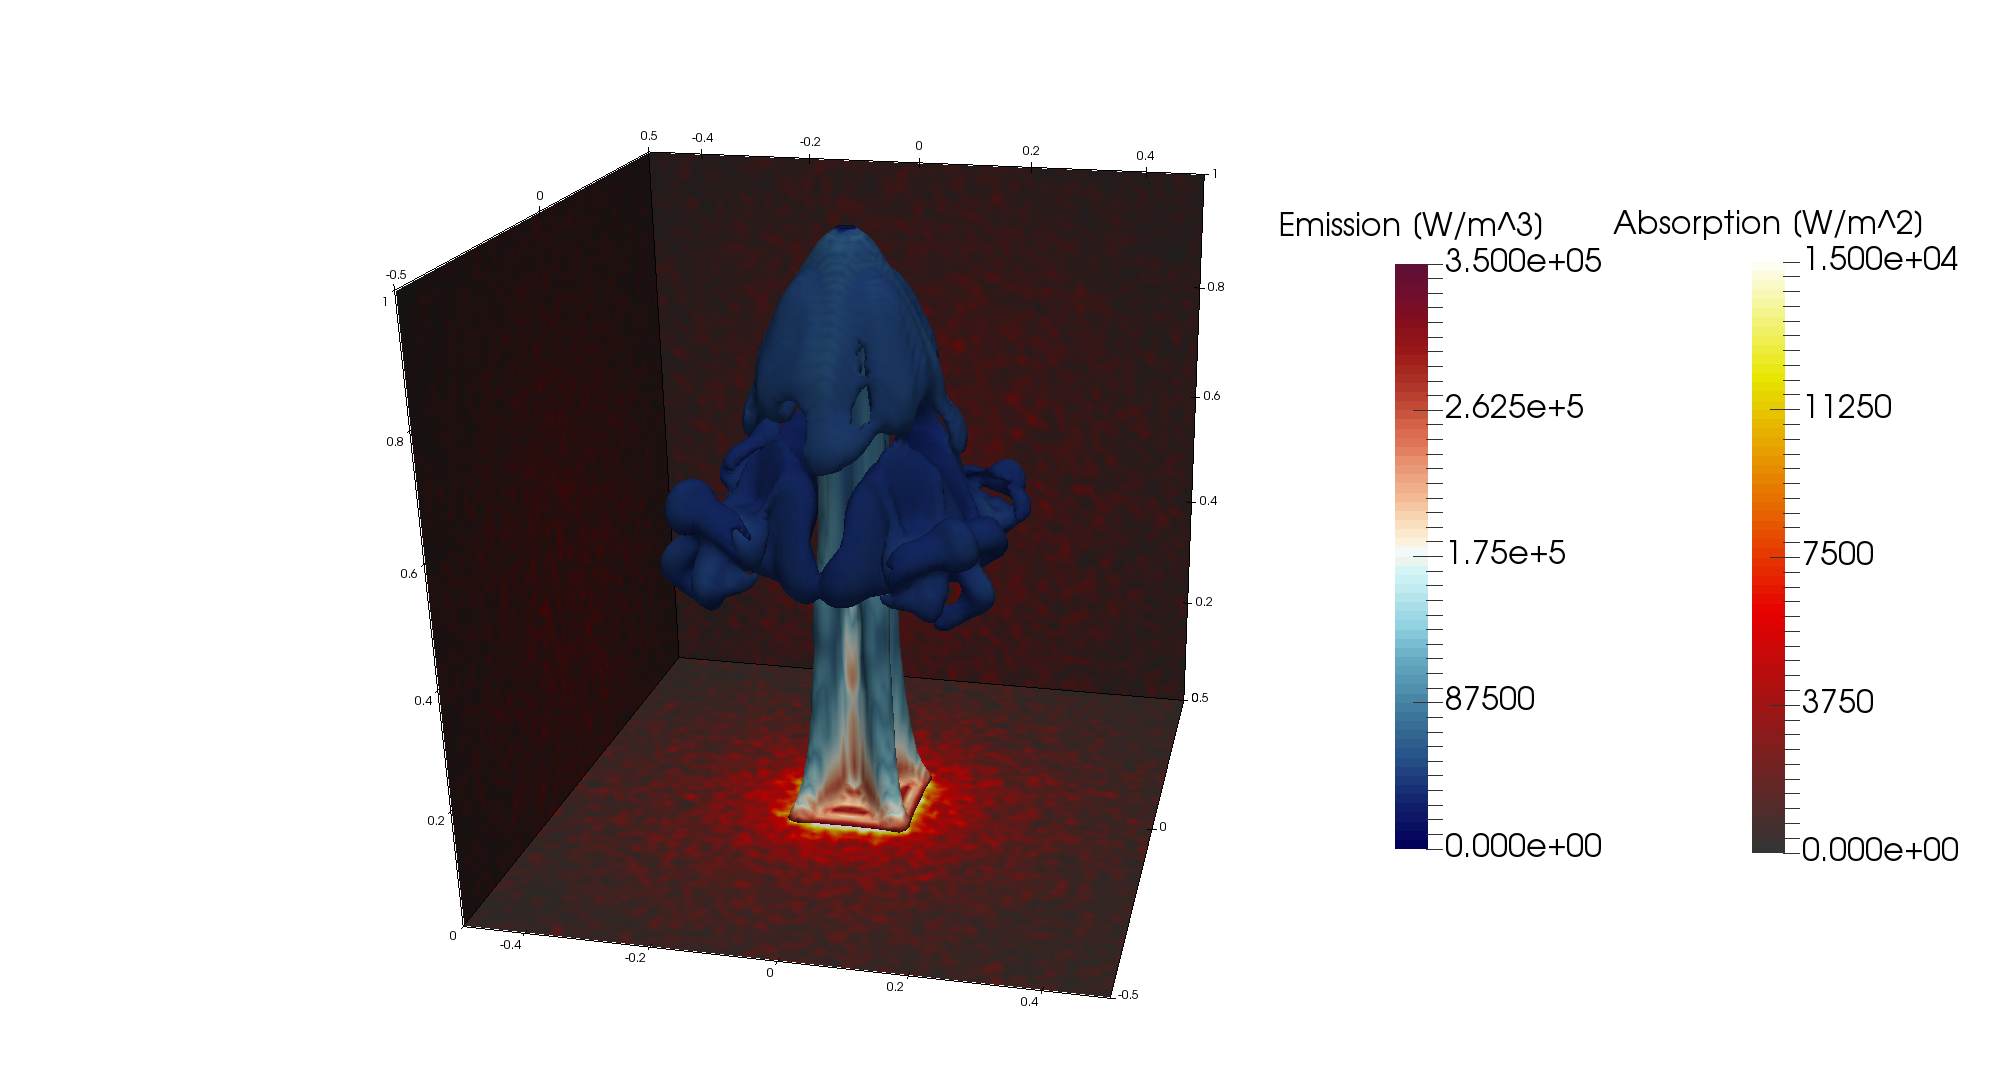
\includegraphics[width=\linewidth]{figures/ch4/radiation_contours.png}
\caption{Isosurface of 0.03 CO$_2$ mass fraction colored by radiative emission. Wall coloring represents wall radiative heat flux.}
\label{fig:PoolFire_radiationcontours}
\end{figure}

\subsubsection{Single Timestep}
A single timestep from the original smallPoolFire3D simulation is extracted, and radiation is simulated.
In order to better understand the influence of radiation within the flame, figure \ref{fig:PoolFire_quadcomparison} displays four relevant parameters for the radiation calculation within the frozen field analysis. 
The contours of temperature show two sides of a hollow cylinder of reacting flow billowing upwards as a result of the buoyant force induce on the lower-density regions.
The top-section of the mushroom contains an  flame-front which, towards the outer regions, slowly decreases in temperature and intensity as a result of momentum and molecular exchange with the surrounding quiescent region through viscous and diffusive effects.
High temperature regions correlate strongly with the points of high emission, and the wings of the mushroom show a much stronger decay in emission as a result of the fourth power dependence of radiative emission with temperature.

Absorption visually appears to correlate much more closely with the Planck-mean absorption coefficient than temperature. Absorption is maximized near the entrance region of the flame, and maintains its strength throughout the tight upwards-moving stream of fluid.
The significant drop in Planck-mean absorption coefficient with radiative absorption in the non-reacting regions of the flow suggests that the flame is responsible for the bulk of radiative re-absorption. 

In total, net radiative emission equals $10541.5044$ Watts, where $1469.4406$ Watts are re-absorbed into the medium, and $9072.0639$ Watts escape to the walls. This results in approximately 14\% of radiative emission being re-absorbed primarily in the flame-region, as suggested previously. 
The maximum volumetric radiative energy loss for any computational cell is -$1.081$ W. In comparison, the maximum volumetric source through chemical reaction was $14.08$ Watts.

\begin{figure}
\centering
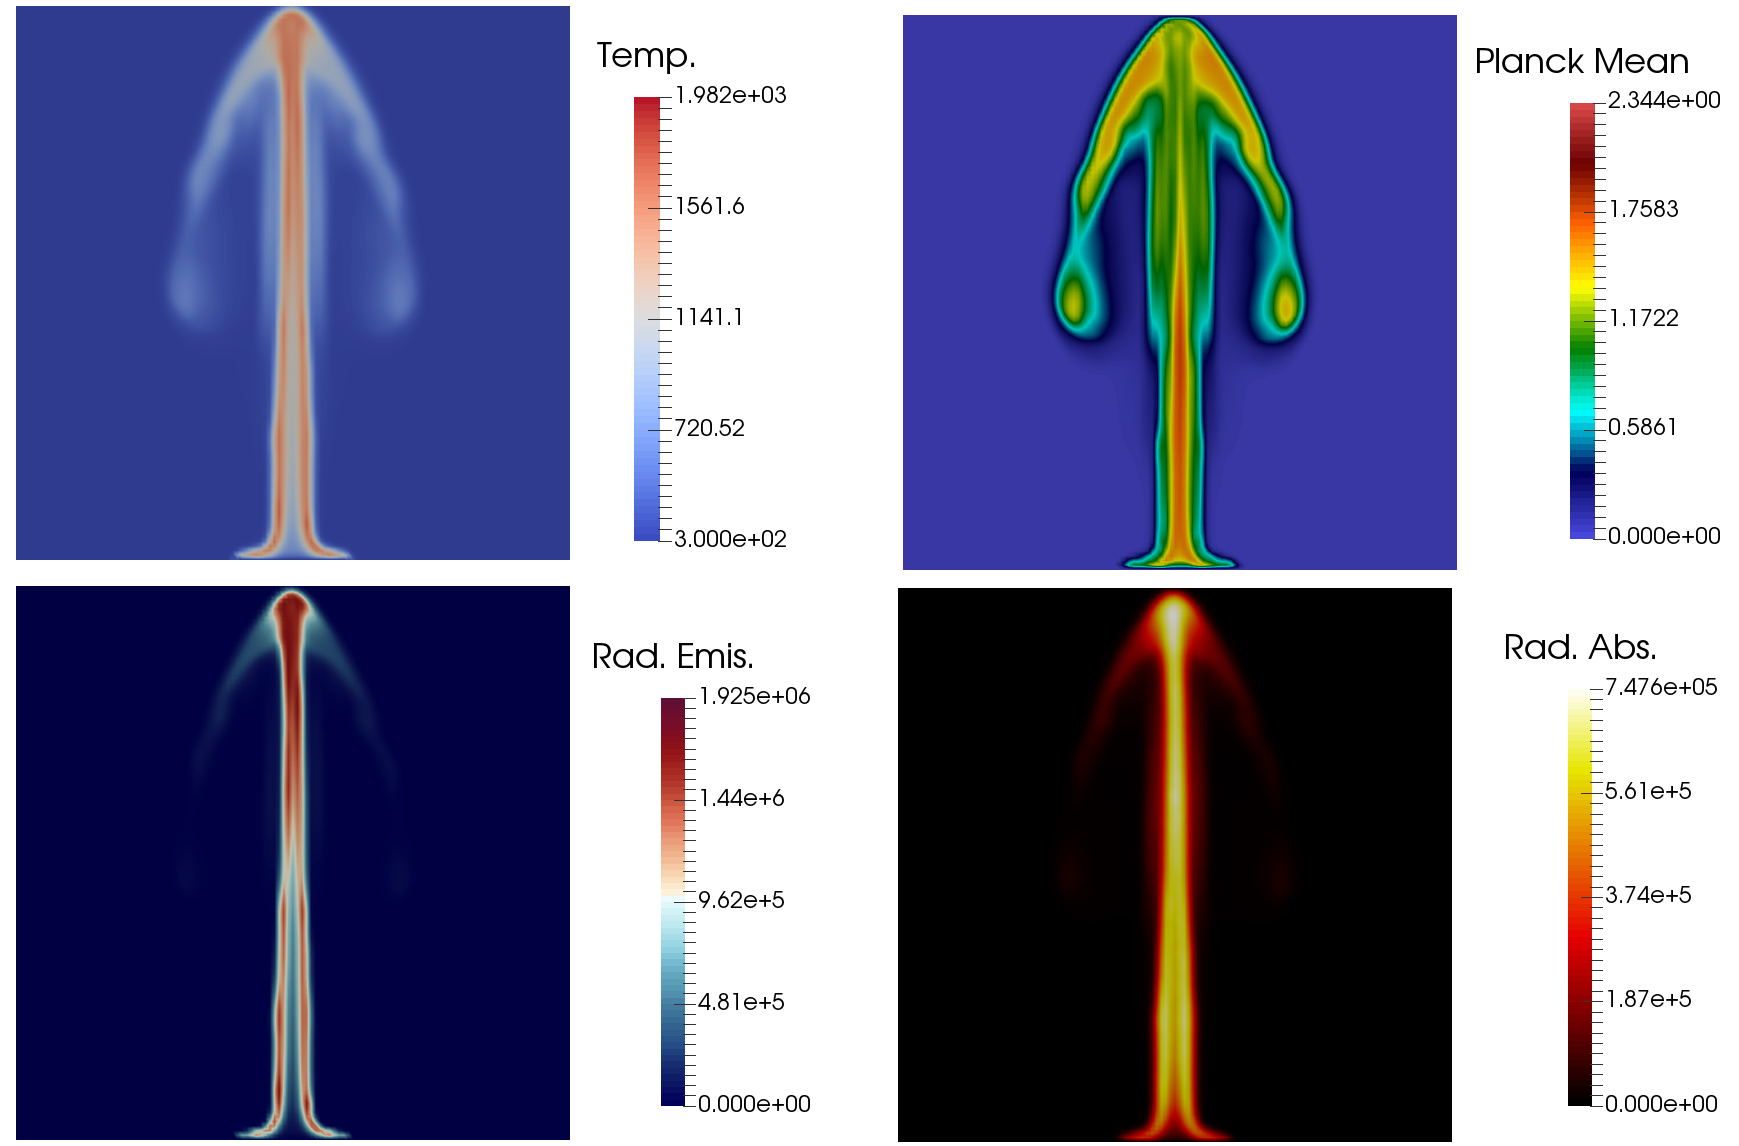
\includegraphics[width=0.9\linewidth]{figures/ch4/PoolFire_quadcomparison.png}
\caption{Mid-plane contours of four relevant parameters to the radiation calculation in the pool fire. Temperature is in Kelvin, Planck Mean absorption coefficient is in m$^{-1}$, and radiative emission and absorption are in W/m$^3$.}
\label{fig:PoolFire_quadcomparison}
\end{figure}

Figure \ref{fig:PoolFire_lineplot} shows various normalized parameters along the center-line of a gray-simulated flame. 
Normalized temperature and product species mass fractions rise with increasing distance from the bottom surface, indicating reaction progression. 
The volumetric emission and negative of radiative volume source (emission – absorption) appear to match as a result of the relatively weak influence of absorption.
The Planck Mean absorption coefficient increases, then decreases despite the monotonically increasing mass fractions of the radiatively participating species (CO$_2$ and H$_2$O). This happens as a direct result of the increase in temperature. 
The influence of temperature on absorption coefficient is complex, but for these conditions the rotation partition function of molecular energy states of the participating species is responsible for the decrease of absorption coefficient at this temperature range~\cite{Modest2013RadiativeTransfer}.
Absorption follows the trend of planck-mean absorption coefficient, as expected for an gray model.

Figure \ref{fig:PoolFire_lineplot_nongray} displays the same normalized parameters in a LBL-accurate Pool-fire simulation. The contributions of CO$_2$ and H$_2$O are considered, but not soot.
The most notable changes are the inversion of the radiative absorption profile. Absorption now increases with height in the flame. Line-by-line accuracy means that the rate of absorption is decided by the wavelength of the ray.
This results in an increase of re-absorption as the rays with wavelengths of high rates of absorption are also preferentially selected for during the random wavenumber selection process. Thus results in a net increase of radiative re-absorption from $14$\% for the gray flame to $58$\% for the non-gray flame.
The resulting negative radiation source contour shown in fig. \ref{fig:PoolFire_lineplot_nongray} also reflects this change by showing a slight degree of absorption towards the lower-sections of the flame.

\begin{figure}[!ht]
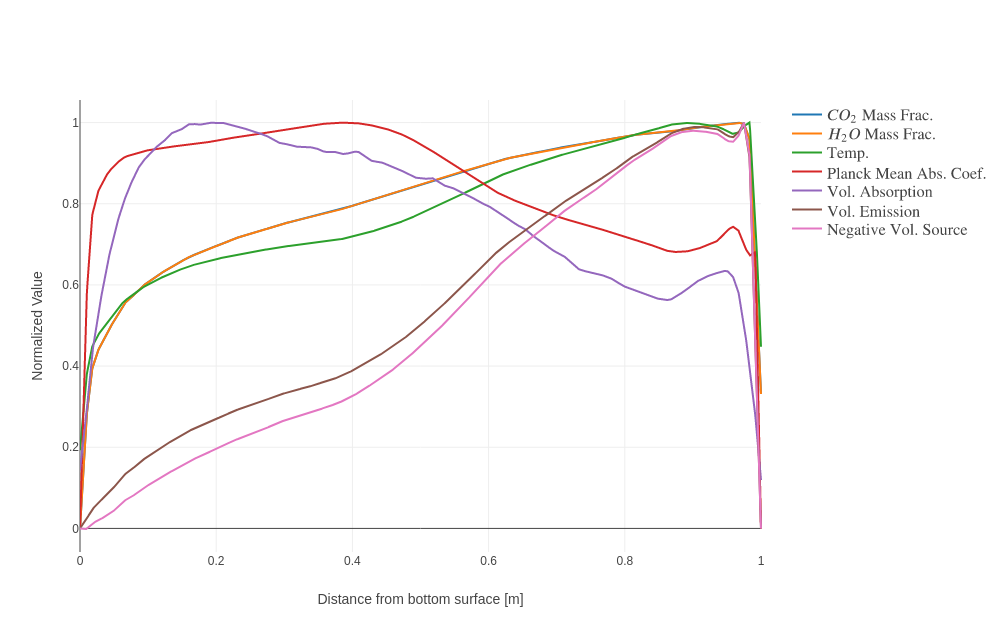
\includegraphics[width=\linewidth]{figures/ch4/line_plot.png}
\caption{Various parameters along the center-line of a gray flame. Values normalized by maximum values along the sampled line.}
\label{fig:PoolFire_lineplot}
\end{figure}


\begin{figure}[!ht]
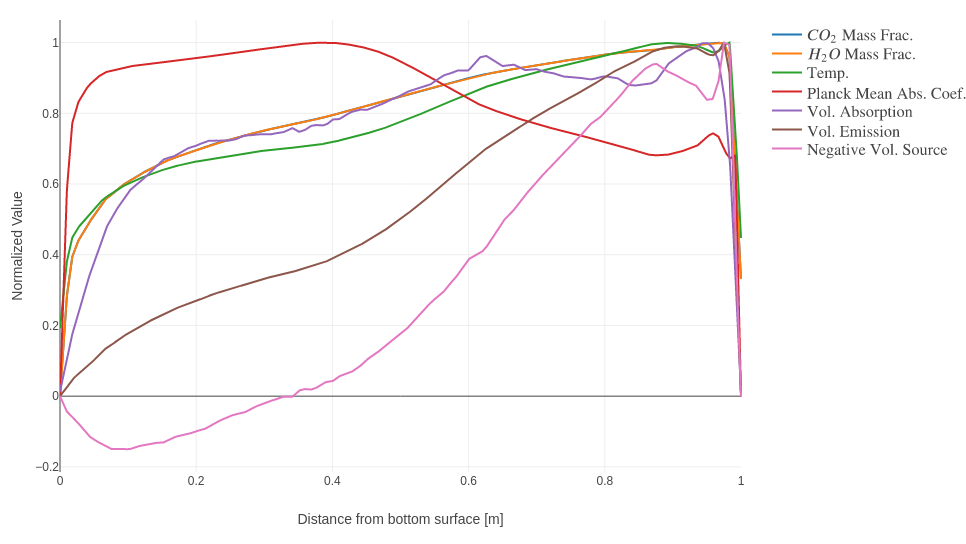
\includegraphics[width=\linewidth]{figures/ch4/line_plot_nongray.png}
\caption{Various parameters along the center-line of a non-gray flame. Values normalized by maximum values along the sampled line.}
\label{fig:PoolFire_lineplot_nongray}
\end{figure}

\subsubsection{Time-accurate simulation}
The same pool-fire is simulated from initial conditions until 4 seconds of physical time.
The simulation is run with line-by-line accurate non-gray emission, and radiation source terms are updated each simulation time-step. Chemistry is infinitely-fast, and the case setup is identical to that of the frozen-field analysis.
Several time-steps of the simulation are present in fig. REF. The pool fire is shown to first appear as a mushroom up from the inlet, the reacting, billowing cloud rises upwards, and finally exits through the top boundary of the domain.
The pool fire periodically fluctuates according to a \textit{puffing period}. These oscillations are buoyancy driven and result in turbulent eddies and substantial cooling of the flame as it mixes with the oxidizer.

Radiation contributes significantly to the reduction of flame temperature, and therefore has a significant effect on the density-driven buoyant forces fluctuating the flame profile. 
Figure \ref{fig:PoolFire_withandwithoutrad} compares the center-line temperature of the pool fire for a simulation without radiation, with the gray OpenFOAM DOM radiation solver, and the gray MCRT model. Significant variations in temperature are apparent, up to $600$K at locations far from the inlet.


\begin{figure}
\centering
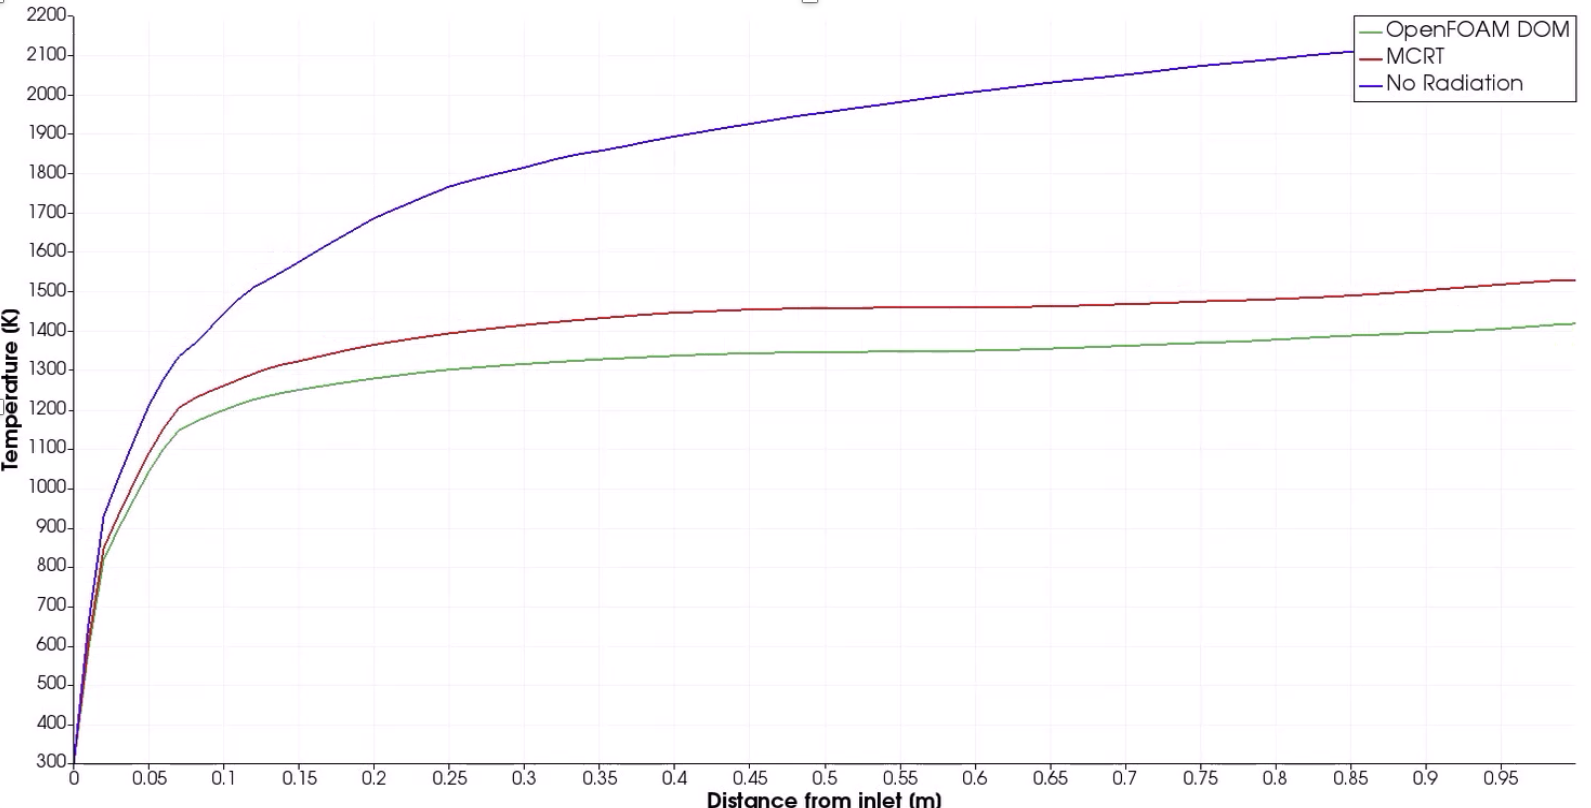
\includegraphics[width=1\linewidth]{figures/ch4/PoolFire_WithandWithoutRadiation.png}
\caption{Comparison of center-line temperature profiles of various simulations of the pool fire.}
\label{fig:PoolFire_withandwithoutrad}
\end{figure}

\subsection{Profiling}
\subsubsection{Single time-step}
The run-times of various sections of the radiation solver are presented in fig. \ref{fig:PoolFire_profiling} and \ref{fig:PoolFire_profiling_CPU} for both CPU and GPU simulations. Simulations are conducted with adaptive emission using a total of 3,429,003 rays.
CPU ray-tracing is completed using 30 CPU processes. 

For both CPU and GPU simulations, the runtime is dominated by the loading of the non-gray database, which is over a gigabyte in size. 
The tracing region is proportionally smaller on the GPU as a result of the significant speedup when conducting raytracing in a SIMD-favorable architecture.
The loading process consists of first loading the data into memory, initializing the representative data structures, conducting various sanity checks on the database to ensure proper loading, and deep copying the data onto the GPU, if present.
Numerical time-step comparisons are present in table \ref{table:PoolFireTimestep_runtime_table_1rpc}.

\begin{figure}
\centering
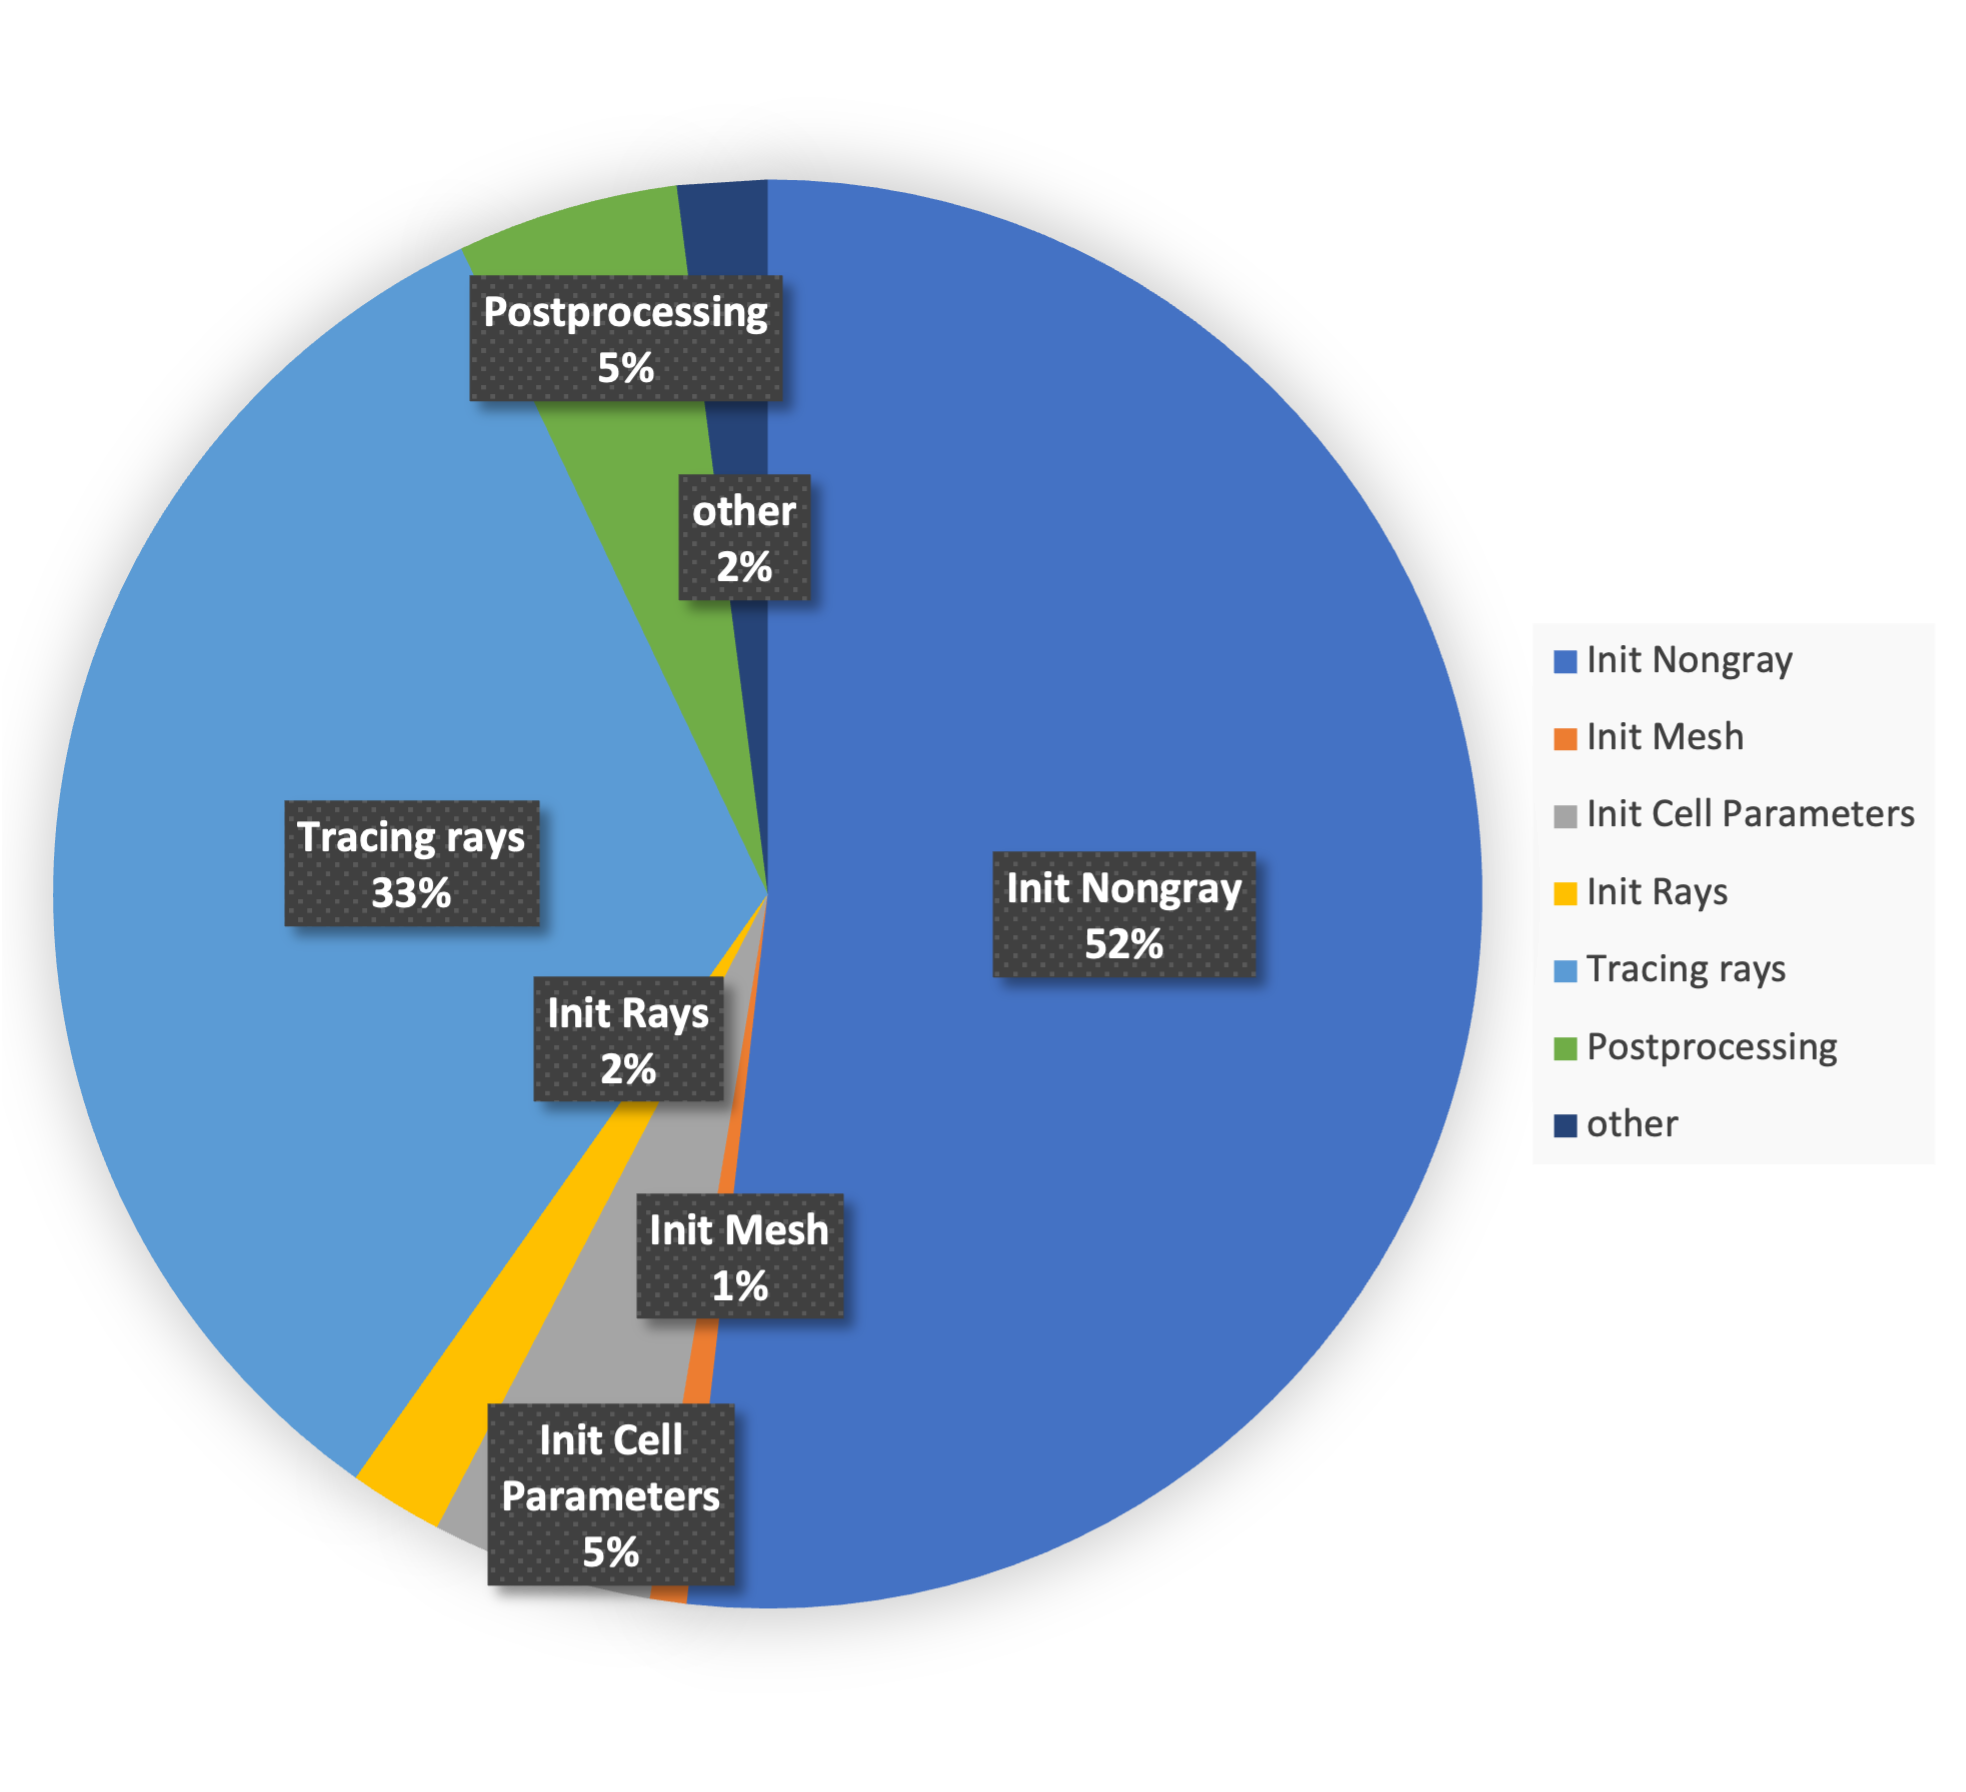
\includegraphics[width=0.675\linewidth]{figures/ch4/PoolFire_profiling_OnetimestepGPU.png}
\caption{Profiling results for the GPU}
\label{fig:PoolFire_profiling}
\end{figure}

\begin{figure}
\centering
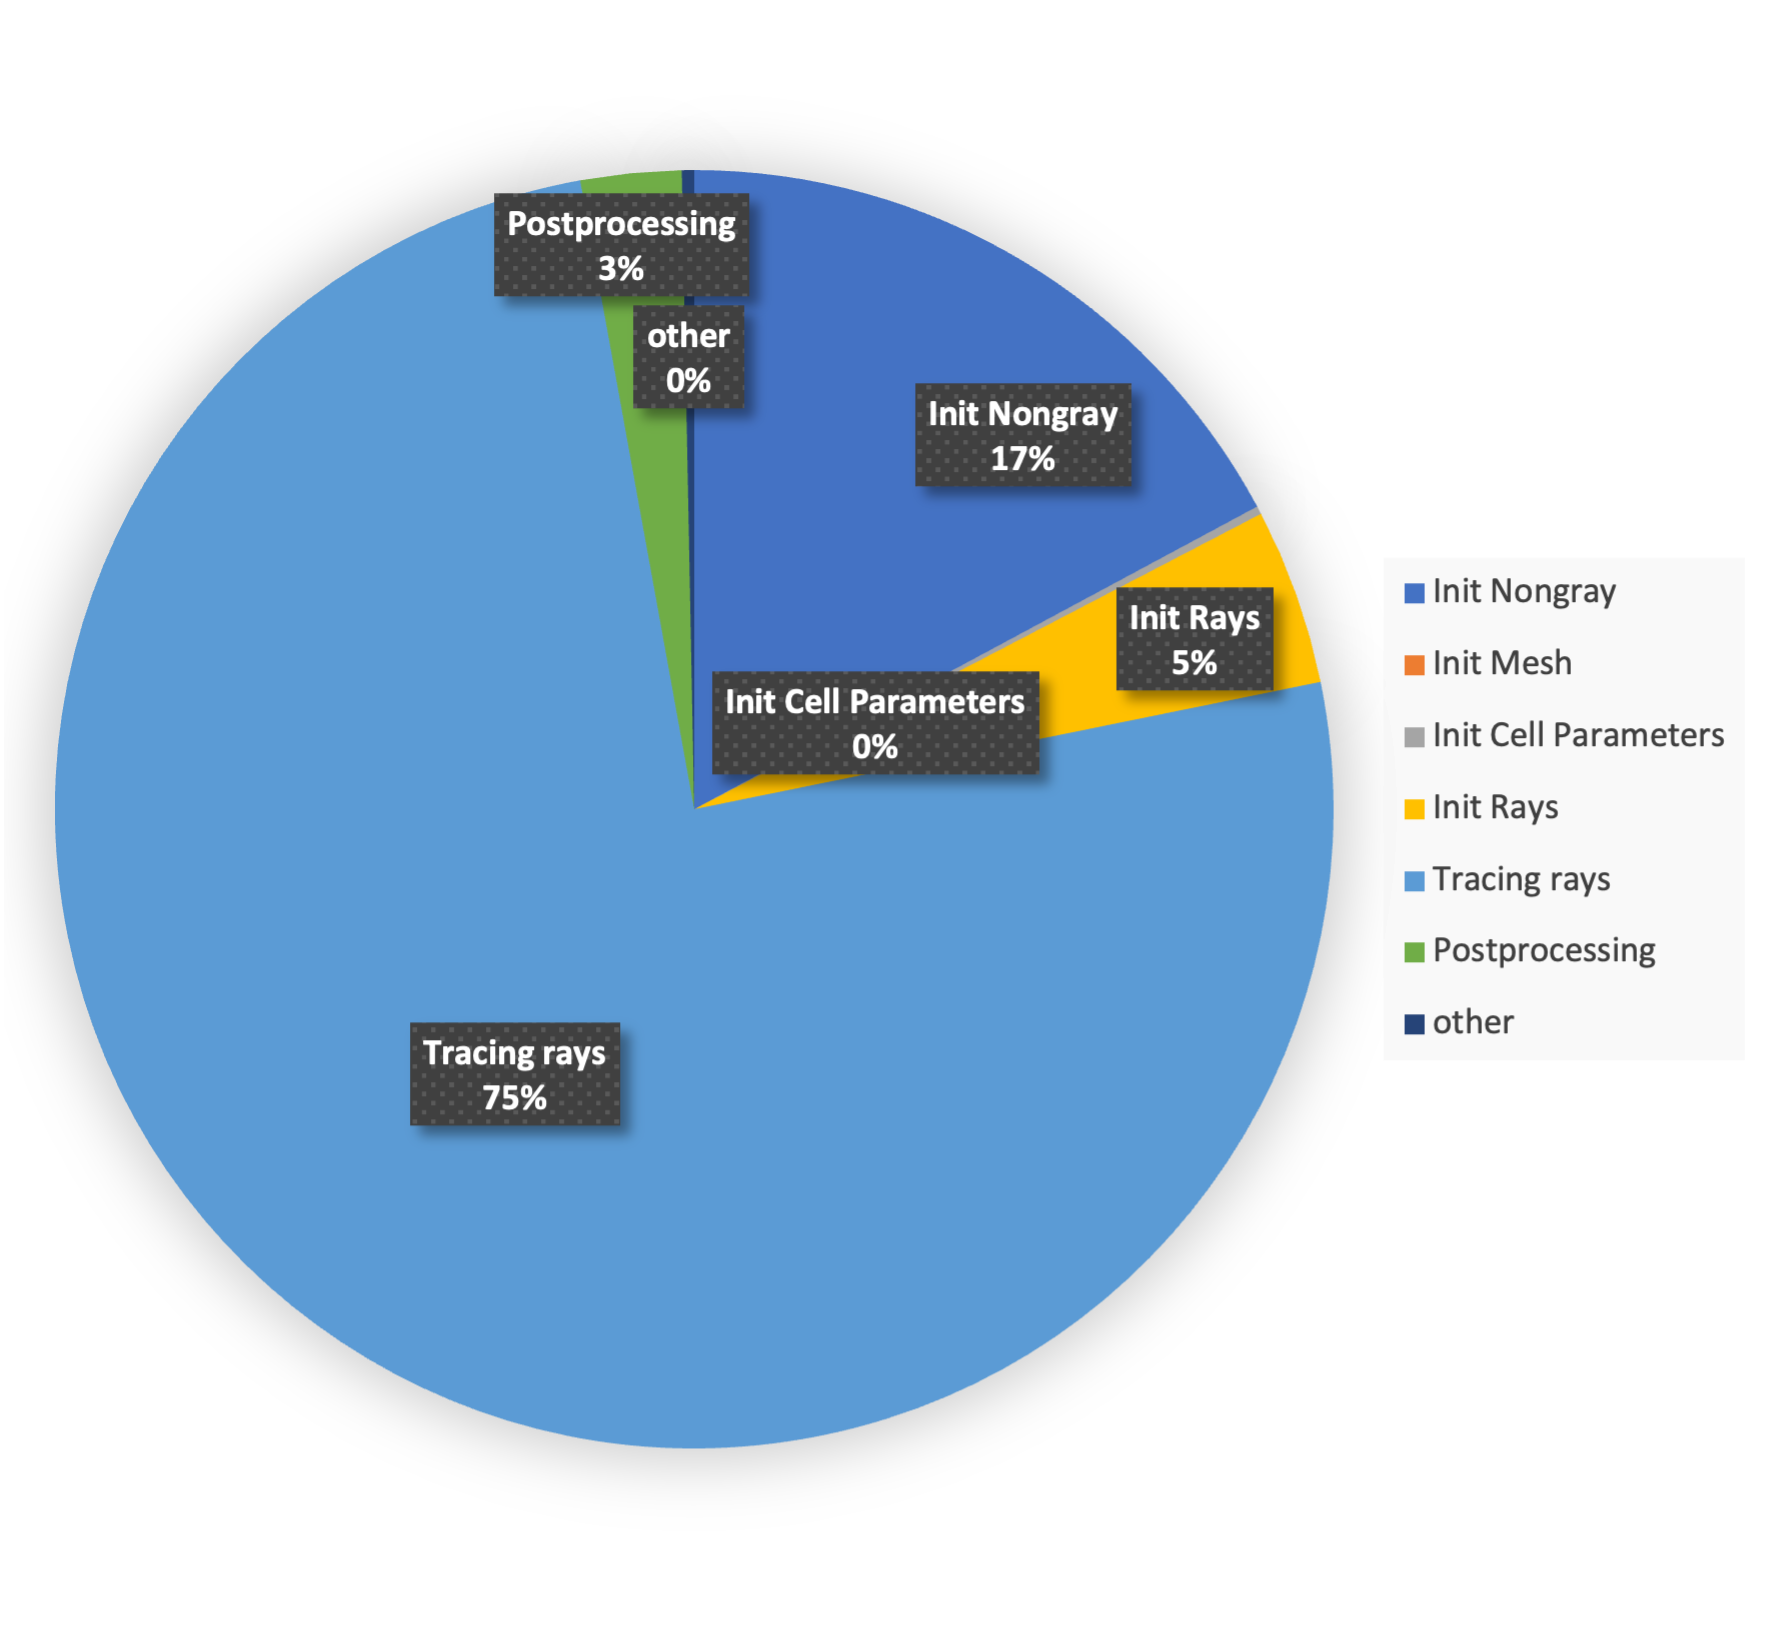
\includegraphics[width=0.675\linewidth]{figures/ch4/PoolFire_profiling_OnetimestepCPU.png}
\caption{Profiling results for the CPU.}
\label{fig:PoolFire_profiling_CPU}
\end{figure}

\begin{table}[h!]
\centering
\caption{Single time-step runtime profiling.}
\begin{tabular}{||c c c c c||} 
 \hline
 Parallel Variation & Init non-gray & Tracing rays & Init cell parameters & Total \\ [0.5ex] 
 \hline\hline
 30 CPU processors & 0.997s & 4.38s & 0.0119s & 5.81s \\
 GPU & 2.25s & 1.44s & 0.218s & 4.34s \\ 
 \hline
\end{tabular}
\label{table:PoolFireTimestep_runtime_table_1rpc}
\end{table}

\subsubsection{Time-accurate simulation}
Time accurate simulations are  conducted with adaptive emission, totalling approximately 3,400,000 rays emitted and traced per time-step.
Both CPU and GPU versions were run for four seconds of simulation time. Mean and standard deviations of run-times are presented in table \ref{table:PoolFireTransient_runtime_table_1rpc}. 

For the CPU-run case, radiation encompassed approximately 37\% of the runtime for each timestep, on average. The detailed profiling results featured in figure \ref{fig:PoolFire_profiling_CPU} can be considered roughly consistent across the various time-steps of the time-accurate simulation.
It should be noted that both the non-gray database and CFD mesh are re-initialized every time-step, resulting in significantly increased run-time. Future work will include initializing these components at the beginning of the simulation to prevent the unnecessary additional runtime.
After these changes, the overall radiation runtime will target $6.723$s, or $33$\% of the total runtime.
Identically, the GPU runtime will target $3.07$s, or $21$\% of the total runtime per timestep.

\begin{table}[h!]
\centering
\caption{Mean runtime contribution of radiation per timestep compared to total runtime. Standard deviations are presented in parenthesis. List CPU runtimes consist of radiation parallelized on 30 CPU processors, and CFD calculation occuring on 1 processor. GPU runtimes consist of radiation running on the GPU and CFD calculated using 1 CPU processor.}
\begin{tabular}{||c c c c||} 
 \hline
 Parallel Variation & Radiation Execution & Total Execution & Percent contribution \\ [0.5ex] 
 \hline\hline
 30 CPU processors & 8.1s($\pm{}$0.58s) & 21.7s($\pm{}$0.84s) & 37.4\%($\pm{}$2.10\%) \\ 
 GPU & 4.7s($\pm$0.28s) & 16.2s($\pm$2.21)s & 29.4\%($\pm$2.30\%) \\
 \hline
\end{tabular}
\label{table:PoolFireTransient_runtime_table_1rpc}
\end{table}


\section{Pratt \& Whitney Aeronautical Combustor}
A three dimensional Pratt \& Whitney combustor \textbf{(Block C)}? geometry was next tested for verification and profiling of the present radiation model. Solver profiling is presented alongside general observations regarding the effects of radiation within the system.
The combustor geometry follows a Rich-Quench-Lean (RQL) configuration, an optimal design for both emissions and stability.
A single time-step from an LES of the combustor was taken for a frozen-field analysis. 
The combustor geometry is constructed to for highly turbulent flow with a high degree of separation to allow for a sufficiently stabilized flame.
A re-circulation zone immediately behind the inlet section induces a swirl which facilitates mixing of the reactants, and a downstream dilution hole results in a complex chemical mixing process for the remaining reactions to occur in a fuel-lean condition. This results in a more complex profile of radiation throughout the fluid and the walls.
The resulting influences of radiation within the fluid and along the walls are non-monotonic with respect to distance from the inlet, and especially with consideration of the influences of non-gray emission and absorption. 
All presented parameters are normalized by median values obtained through the computational cells or faces.


\subsection{Case setup}
The combustor geometry consists of one slice of the annular combustor. The domain is meshed into a grid of 16,373,876 hexahedral cells of varying shapes and sizes. 
Radiation is modeled with adaptive emission, as discussed in section \ref{section:SmallPoolFlame}, and specularly reflective boundary conditions are imposed on the periodic boundaries.
The effects of soot, spectral emission patterns, and wall-incident radiation were all captured within the model, and detailed account of these effects alongside profiling of the various parallel implementations of the model are presented as demonstration.
Contributions from the three primary emitting and absorbing chemical species are accounted for: CO$_2$, H$_2$O, and CO, as well as the influences of soot are also accounted for.
The effects of liquid fuel spray on ray-scattering and absorption and all turbulence-radiation interactions are neglected.

\subsection{Results}

\subsubsection{Radiative Emission}
It is of interest to first investigate the radiative emission characteristics of the combustor.
Equation \ref{eq:RadEmis} (repeated in volumetric form in eq. \ref{eq:RadEmis2}) defines the influence of both Planck mean absorption coefficient $\kappa{}$ and temperature $T$ on volumetric radiative emission.
\begin{equation}
    Q_{emi}=4\kappa{}_{p}n^2\sigma{}T^4
    \label{eq:RadEmis2}
\end{equation}
Where the refractive index $n$ is assumed constant. 
The volumetric emission is a function of both Planck mean absorption coefficient and temperature. It is important to note, however, that Planck mean absorption coefficient is itself a function of temperature, in addition to the chemical composition of the mixture. 

\textbf{\checkmark Figure: 3 Scatter plots of emission, kplanck, and fvSoot vs temperature}

Parameters from computational cell data are displayed in normalized form in fig. \ref{fig:PW_Scatterplot_emission}. 
Suprisingly, radiative emission displays a non-monotonic trend with respect to temperature. The scaling reflects the expected fourth-order nature before the normalized temperature value of $0.7$, but decreases sharply as temperature continues to increase.
At this point, the contribution of temperature to radiative emission is superseded by the decrease in Planck-mean absorption coefficient.
This is evident in figure \ref{fig:PW_kplanck_scatter}.
Between temperatures of T=$0.4$ and $0.7$, $\kappa{}_p$ shows a gradual decline. After a value of T=$0.7$, however, $\kappa{}_{p}$ begins to decrease much more rapidly towards $0$. 
The various contributions of the $\kappa{}$ are presented in eq. \ref{eq:Kplanck_definition}.
\begin{equation}
    \kappa{}_p=f_{v,soot}\kappa{}_{soot}+X_{CO_2}\kappa{}_{CO_2}+X_{H_2O}\kappa{}_{H_2O}+X_{CO}\kappa{}_{CO}
    \label{eq:Kplanck_definition}
\end{equation}
Where $f_{v,soot}$ is the soot volume fraction, and $X_i$ is the mole fraction of species $i$.
The contributions of each of the terms in equation \ref{eq:Kplanck_definition} are presented in fig. \ref{fig:PW_kplanck_contributions}. All values are normalized by the contributions of soot.
It is evident that soot plays the most significant role in defining the absorption coefficient at present conditions. Additionally, the sharp decrease of Planck mean absorption coefficient present in fig. \ref{fig:PW_Scatterplot_kplanck} at T=$0.7$, also presents itself in the temperature profile of soot volume fraction in fig. \ref{fig:PW_Scatterplot_soot}.
This sudden drop represents a crossover point. At this temperature, soot particles are consumed rapidly by the gas, and the resulting radiative emission rapidly decreases.

\subsubsection{Radiative Absorption}
As mentioned in chapter \ref{chapter:Importance}, the redistribution of thermal energy from radiation is significant for multiple reasons: radiation can produce changes in the fluid dynamics, turbulence, wall heat flux, and the chemical production of pollutants.
The Pratt \& Whitney combustor displays a relevant degree involvement of radiative absorption to each of these characteristics.

Figure \ref{fig:PW_WallAverages} presents the averaged wall heat flux for the inner diameter (ID) and outer diameter (OD) surfaces of the annular combustor slice. 
The walls are assumed to be cold and black; they absorb all incident radiation and re-emit a negligible amount. 
Wall-incident radiation increases throughout the rich-burn section of the combustor, reaches a local maximum just before the dilution holes, and decreases throughout the lean-burn section.
This corroborates the results presented by \citet{Gamil2020AssessmentChamber}, where the fuel-rich section of the flame was shown to emit highly and increase the temperatures of the combustor walls.

\textbf{\checkmark Figure: Average wall heat flux profile as a function of distance from the inlet}

To analyze the contribution of non-gray absorption to the flame, gray and non-gray wall heat flux is presented in fig. \ref{fig:WallHeatFlux_GrayVsNongray}.
Both ID and OD walls see up to 50 to 60\% decreases in wall heat flux when the line-by-line radiation model is introduced. Decreases diminish slightly in the fuel-rich part of the combustor to 30 to 40\%, but remain substantial.
Net percent differences in wall heating is presented for various boundaries in fig. \ref{table:PW_GrayVsNonGray}.
The decrease in radiative transmission to the walls is a direct result of the increased re-absorption within the flame. 
The introduction of non-gray modeling causes increased attenuation of radiation. Changes in radiative re-absorptions are presented for both soot and 


\textbf{$\times$ Figure: gray vs non-gray averaged heat flux values in the fluid}

\begin{table}[h!]
\centering
\begin{tabular}{||c c||} 
 \hline
 Boundary & Percent Decrease \\ [0.5ex] 
 \hline\hline
 OD Wall & 6 \\ 
 ID Wall & 7  \\
 Turbine & 545  \\
 Inlet & 545  \\ [1ex] 
 \hline
\end{tabular}
\caption{Percent differences in incident radiative power between gray and non-gray radiation models.}
\label{table:PW_GrayVsNonGray}
\end{table}

The overall budgeted contributions to wall heat flux are diagrammed in fig. \ref{fig:PW_emission_contributions} across the emission spectrum.
The intermittent nature of the emission from the molecules is reflected by the accounted contributions of CO$_2$, H$_2$O, and CO. The emission of soot is more continuous throughout the spectrum, as expected.
Overall, soot contributes the majority of emission from the flame, with emission occurring generally at more moderate temperatures, as previously discussed.

\textbf{\checkmark Figure:Budgeted contributions of species and soot across the spectrum.}

\subsection{Profiling}
The new MCRT implementation displayed a significant speedup compared to the established fortran model. A comparison of runtimes is present in fig. \ref{table:PW_runtime_table}

\begin{table}[h!]
\centering
\begin{tabular}{||c c c c||} 
 \hline
 Variation & MCRT-Fort & MCRT-Kokkos & MCRT-ArborX \\ [0.5ex] 
 \hline\hline
 Gray & 5770s     & 2308 & 57  \\ % TODO
 Non-Gray & 5770s & 3000 & 78 \\ [1ex] 
 \hline
\end{tabular}
\caption{Runtime comparisons for the Pratt \& Whitney combustor geometry.}
\label{table:PW_runtime_table}
\end{table}


- Runtime gray

- Runtime non-gray


